\documentclass{article}
\usepackage[utf8]{inputenc}
\usepackage[brazil]{babel}
\usepackage{graphicx}
\usepackage{amsmath, amssymb}
\usepackage{hyperref}
\usepackage{float}
\usepackage[a4paper, margin=1in]{geometry} 
\usepackage{setspace}
\onehalfspacing


\title{Fundamentos de Probabilidade e Estatística para Ciência de Dados}
\author{Resumo das aulas do Prof. Dr. Francisco Rodrigues (ICMC-USP)}
\date{Agosto de 2025}

\begin{document}

% Capa personalizada
\begin{titlepage}
    \centering
    \vspace*{3cm}
    {\scshape\LARGE Universidade de São Paulo \par}
    \vspace{1cm}
    {\scshape\Large Instituto de Ciências Matemáticas e de Computação\par}
    \vspace{2.5cm}
    {\huge\bfseries Fundamentos de Probabilidade e Estatística para Ciência de Dados\par}
    \vspace{1cm}
    {\Large Resumo das aulas do Prof. Dr. Francisco Rodrigues\par}
    \vfill
    {\Large Bruna Zamith Santos\par}
    \vspace{0.5cm}
    {\large Agosto de 2025\par}
\end{titlepage}

% Sumário
\tableofcontents
\newpage

\section{Teoria dos Conjuntos}
Sejam os conjuntos:
\[
A = \{1, 2, 4, 9\}, \quad B = \{3, 7, 9\}
\]

\begin{itemize}
  \item União: $A \cup B = \{1, 2, 3, 4, 7, 9\}$
  \item Interseção: $A \cap B = \{7, 9\}$
  \item Complementar de $B$: $B^C = \{1, 2, 4\}$
  \item Complementar de $A$: $A^C = \{3, 7\}$
  \item Espaço amostral ($\Omega$): É o conjunto de todos os resultados possíveis de um experimento aleatório. Exemplo: $\Omega = \{1, 2, 3, 4, 5, 6\}$, ao lançar um dado.
  \item Evento ($A$): É um subconjunto do espaço amostral. Exemplo: $A = \{2, 4, 6\}$
  \item Evento impossível ($\emptyset$): É um evento que nunca ocorre.
  \item Evento certo ($\Omega$): É o evento que sempre ocorre.
  \item $A \cup B$: É o evento que ocorre se $A$ ou $B$ (ou ambos) ocorrerem.
  \item $A \cap B$: É o evento que ocorre se $A$ e $B$ ocorrerem ao mesmo tempo.
  \item $A^C$: É o evento que ocorre se $A$ não ocorre.
  \item Eventos mutuamente exclusivos: Quando $A \cap B = \emptyset$.
\end{itemize}

\section{Experimento Aleatório}
Um experimento aleatório é um experimento que pode ser repetido inúmeras vezes sob as mesmas condições, sendo o seu resultado incerto.

\section{Conceitos de Probabilidade}
Sejam $\Omega$ o espaço amostral e $A$ um evento em $\Omega$. Então, uma função $P(\cdot)$ é denominada probabilidade se satisfaz:
\begin{itemize}
    \item $0 \leq P(A) \leq 1$, $\forall A \in \Omega$ 
    \item $P(\Omega) = 1$
    \item Se $A_1, A_2, \dots$ forem eventos mutuamente exclusivos, isto é, $A_i \cap A_j = \emptyset$, $\forall i \neq j$, então:
    $$
    P\left( \bigcup_{i=1}^{\infty} A_i \right) = \sum_{i=1}^{\infty} P(A_i)
    $$
\end{itemize}

Se um experimento aleatório tiver $n(\Omega)$ resultados mutuamente exclusivos e igualmente possíveis, e se um evento $A$ conter $n(A)$ desses resultados, a probabilidade de ocorrência desse evento é definida por:
    $$
    P(A) = \frac{n(A)}{n(\Omega)} = \frac{|A|}{|\Omega|}
    $$

Sejam $A$ e $B$ eventos em um mesmo espaço amostral, então:

\begin{itemize}
  \item $P(\emptyset) = 0$
  \item $P(A) = 1 - P(A^C)$
  \item Se $A \subseteq B$, então $P(A) \leq P(B)$
\end{itemize}

\subsection{Probabilidade Frequentista}
A probabilidade de um evento é igual à sua frequência de ocorrência em um grande número de experimentos:
    $$
    P(A) = \lim_{n \to \infty} \frac{n_A}{n}
    $$,
onde $n_A$ é o número de vezes que o evento $A$ ocorre em $n$ experimentos.

\subsection{Probabilidade de União de Dois Eventos}
Para dois eventos $A$ e $B$ em um mesmo espaço amostral:
    $$
    P(A \cup B) = P(A) + P(B) - P(A \cap B)
    $$

\subsection{Probabilidade Condicional}
Sejam dois eventos $A$ e $B$ em um mesmo espaço amostral $\Omega$.  
A probabilidade condicional de $A$ dado que $B$ ocorreu é definida por:
    $$
    P(A \mid B) = \frac{P(A \cap B)}{P(B)}, \quad \text{com } P(B) > 0
    $$

Assim, $A$ e $B$ são eventos independentes se, e somente se:
    $$
    P(A \cap B) = P(A) \cdot P(B)
    $$

Ou equivalentemente:
    $$
    P(A \mid B) = P(A) \quad \text{e} \quad P(B \mid A) = P(B)
    $$

\subsection{Partições do Espaço Amostral}
Os eventos $B_1, B_2, \dots, B_n$ formam uma partição do espaço amostral $\Omega$ se:

\begin{itemize}
    \item $B_i \cap B_j = \emptyset$, para $i \neq j$, com $i, j = 1, \dots, n$
    \item $\bigcup_{i=1}^n B_i = \Omega$
    \item $P(B_i) \geq 0$, para $i = 1, \dots, n$
\end{itemize}

Seja $A$ um evento no espaço amostral $\Omega$ e seja $B_1, \dots, B_n$ uma partição amostral de $\Omega$. Podemos escrever $A$ considerando tal partição:
    $$
    A = \bigcup_{i=1}^n (A \cap B_i)
    $$
    $$
    P(A) = P\left( \bigcup_{i=1}^n A \cap B_i \right) = \sum_{i=1}^n P(A \cap B_i)
    $$

\section{Lei da Probabilidade Total}
Sejam $B_1, B_2, \dots, B_n$ uma partição do espaço amostral $\Omega$. Então, qualquer evento $A \subseteq \Omega$ pode ser escrito como:
    $$
    P(A) = \sum_{i=1}^n P(A \mid B_i) \cdot P(B_i)
    $$

\section{Teorema de Bayes}
Sejam $B_1, B_2, \dots, B_n$ uma partição do espaço amostral $\Omega$, e $A$ um evento com $P(A) > 0$, então:
    $$
    P(B_i \mid A) = \frac{P(A \mid B_i) \cdot P(B_i)}{\sum_{j=1}^n P(A \mid B_j) \cdot P(B_j)}
    $$

E assim podemos definir:
    $$
    P(A \mid B) = \frac{P(B \mid A) \cdot P(A)}{P(B)}
    $$

\section{Variáveis Aleatórias}
Suponha que lancemos dois dados. O espaço amostral associado ao experimento, sendo os eventos $C$: ``sai uma cara'' e $R$: ``sai uma coroa'', é dado por:

$$
\Omega = \{CC, CR, RC, RR\}
$$

Uma possível variável aleatória associada ao experimento é definida por:
$$
X = \text{``número de caras obtido no experimento''}
$$

\begin{itemize}
    \item Representamos variáveis aleatórias por letras maiúsculas ($X, Y, Z$), enquanto usamos letras minúsculas para indicar os valores das variáveis ($x, y, z$).
    \item Se o número de valores possíveis de uma variável aleatória for finito ou infinito enumerável, dizemos que é uma variável aleatória discreta.
    \item Caso contrário, é uma variável aleatória contínua.
\end{itemize}

A função que atribui a cada valor da variável aleatória sua respectiva probabilidade é chamada de distribuição de probabilidade:
    $$
    P(X = x_i) = p(x_i) = p_i, \quad i = 1,2,3
    $$

A distribuição de probabilidade também é chamada de função massa de probabilidade. E temos que:
    $$
    \sum_{i=1}^{n} P(X = x_i) = 1
    $$

Dizemos que $X$ é uma variável aleatória contínua se existir uma função $f$ denominada função densidade de probabilidade (fdp) que satisfaz:
\begin{itemize}
    \item $f(x) \geq 0, \quad \forall x \in \mathbb{R}$
    \item $\int_{-\infty}^{\infty} f(x) \, dx = 1$
    \item $P(a \leq X \leq b) = \int_{a}^{b} f(x) \, dx
    $, $-\infty < a < b < \infty$
    \item $f(x)$ é uma função com valores positivos e área unitária.
\end{itemize}

Seja $X$ uma variável aleatória discreta ou contínua. A probabilidade condicional de que $X \in S$ dado que $X \in V$ é:
    $$
    P(X \in S \mid X \in V) = \frac{P(X \in S \cap V)}{P(X \in V)}
    $$,
onde $S$ e $V$ são subconjuntos do espaço da variável.

\section{Função de Distribuição}
A função distribuição acumulada ou simplesmente função de distribuição de uma variável aleatória $X$ é definida por:
    $$
    F(x) = P(X \leq x)
    $$

Se discreta:
    $$
    F(x) = \sum_{x_i \leq x} P(X = x_i)
    $$

Se contínua:
    $$
    F(x) = \int_{-\infty}^{x} f(t) \, dt
    $$

Propriedades da função de distribuição:
\begin{itemize}
    \item $0 \leq F(x) \leq 1, \quad F(x) \text{ é não decrescente}$,
    \item $\lim_{x \to -\infty} F(x) = 0, \quad \lim_{x \to +\infty} F(x) = 1$
    \item Caso discreto: $P(a < X \leq b) = F(b) - F(a)$
    \item Caso contínuo: $f(x) = \frac{dF(x)}{dx}$
\end{itemize}

\section{Esperança}
\subsection{Variável Aleatória Discreta}
Seja $X$ uma variável aleatória discreta com distribuição de probabilidade $P(X = x_i)$. O valor esperado (ou esperança matemática) é:
    $$
    E[X] = \sum_{i=1}^{n} x_i \cdot P(X = x_i)
    $$

\subsection{Variável Aleatória Contínua}
Seja $X$ uma variável aleatória contínua com função densidade de probabilidade $f(x)$, então:
    $$
    E[X] = \int_{-\infty}^{+\infty} x \cdot f(x) \, dx
    $$

\subsection{Função de uma Variável Aleatória}
Seja $g(X)$ uma função de uma variável aleatória discreta $X$. Então:
    $$
    E[g(X)] = \sum_{i=1}^{n} g(x_i) \cdot P(X = x_i)
    $$

Seja $g(X)$ uma função de variável contínua com densidade $f(x)$. Então:
    $$
    E[g(X)] = \int_{-\infty}^{\infty} g(x) \cdot f(x) \, dx
    $$

\subsection{Propriedades}
\begin{itemize}
    \item Se $X = c$, onde $c$ é constante, então: $E[X] = E[c] = c$
    \item Se $c$ é constante: $E[cX] = c \cdot E[X]$
    \item Então: $E[aX + b] = a \cdot E[X] + b$
\end{itemize}

\section{Momento}
\subsection{Momento Estatístico}
Seja $X$ uma variável aleatória discreta com valores $x_1, x_2, \dots, x_k$. O momento de ordem $n$ de $X$ é:
    $$
    E[X^n] = \sum_{i=1}^{k} x_i^n \cdot P(X = x_i)
    $$

Se $X$ for contínua:
    $$
    E[X^n] = \int_{-\infty}^{\infty} x^n f(x) \, dx
    $$

\subsection{Momento Central}
Seja $X$ uma variável aleatória.

\begin{itemize}
    \item Se $X$ é discreta, o momento central de ordem $n$ ($n > 0$) de $X$ é:
    $$
    \mu_n = E\left[(X - E[X])^n\right] = \sum_{x_i} (x_i - E[X])^n \cdot P(X = x_i)
    $$
    \item Se $X$ é contínua, então:
    $$
    \mu_n = E\left[(X - E[X])^n\right] = \int_{-\infty}^{\infty} (x - E[X])^n \cdot f(x) \, dx
    $$
\end{itemize}

\section{Variância}
A variância de uma variável aleatória $X$ é definida por:
    $$
    V(X) = \sigma^2 = E\left[(X - E(X))^2\right]
    $$

O desvio padrão é igual à raiz quadrada da variância:
    $$
    \sigma = \sqrt{V(X)}
    $$

Temos a propriedade de que:
    $$
    V(X) = E[X^2] - (E[X])^2
    $$

Seja $g(X)$ uma função da variável aleatória $X$. Então,
    $$
    V[g(X)] = E[g(X)^2] - \left(E[g(X)]\right)^2
    $$

Seja $X$ uma variável aleatória e $a$ e $b$ constantes. Então,
    $$
    V(aX + b) = a^2 \cdot V(X)
    $$

\section{Modelos Probabilísticos (Estocásticos) Discretos}
\begin{itemize}
    \item Os resultados de cada experimento parecem imprevisíveis, mas quando um grande número de experimentos é analisado, surge um padrão.
    \item Não podemos determinar o valor exato do resultado de um experimento, mas sim as probabilidades de cada resultado possível.
\end{itemize}

\subsection{Distribuição Uniforme Discreta}
Seja $X$ uma variável aleatória discreta assumindo os $n$ valores  $\{a, a + c, a + 2c, \ldots, b - c, b\}$,  com $a, b \in \mathbb{R}$, $c \in \mathbb{R}_{> 0}$ e $a < b$.

Dizemos que $X$ segue o modelo uniforme discreto se atribuímos a mesma probabilidade $1/n$ a cada um desses valores.  
Isto é, sua distribuição de probabilidade é dada por:
    $$
    P(X = x) = \frac{1}{n}, \quad x = a, a + c, a + 2c, \ldots, b
    $$
onde:
    $$
    n = 1 + \frac{b - a}{c}
    $$

Então,
    $$
    E[X] = \frac{a + b}{2},
    $$
    $$
    V(X) = \frac{c^2(n^2 - 1)}{12}
    $$

A Figura~\ref{fig:dist_disc_uniforme} apresenta um exemplo de Distribuição Uniforme discreta.

\begin{figure}[H]
    \centering
    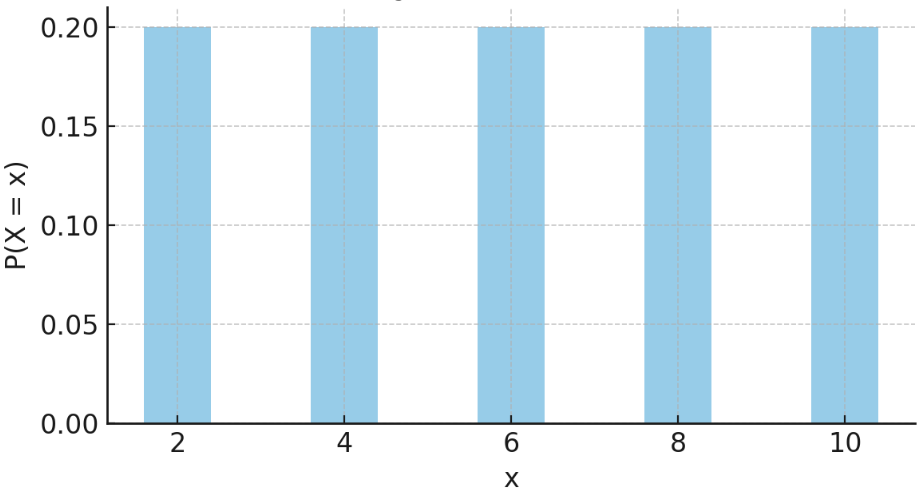
\includegraphics[width=0.6\textwidth]{figuras/dist_disc_uniforme.png}
    \caption{Distribuição Uniforme discreta.}
    \label{fig:dist_disc_uniforme}
\end{figure}

\subsection{Distribuição de Bernoulli}
Dizemos que a variável aleatória $X$ segue o modelo de Bernoulli se atribuímos $0$ à ocorrência de um fracasso ou $1$ à ocorrência de um sucesso, com $p$ representando a probabilidade de sucesso,  
$0 \leq p \leq 1$, e $1 - p$ a probabilidade de fracasso.

A distribuição de probabilidade é dada por:
    $$
    P(X = k) = p^k (1 - p)^{1 - k}, \quad k = 0, 1
    $$

    \begin{center}
    \begin{tabular}{c|cc}
    $X$ & 0 & 1 \\
    \hline
    $P(X = k)$ & $1 - p$ & $p$
    \end{tabular}
    \end{center}

Então,
    $$
    E[X] = p,
    $$
    $$
    V(X) = p \cdot (1-p)
    $$

A Figura~\ref{fig:dist_disc_bernoulli} apresenta um exemplo de Distribuição de Bernoulli.

\begin{figure}[H]
    \centering
    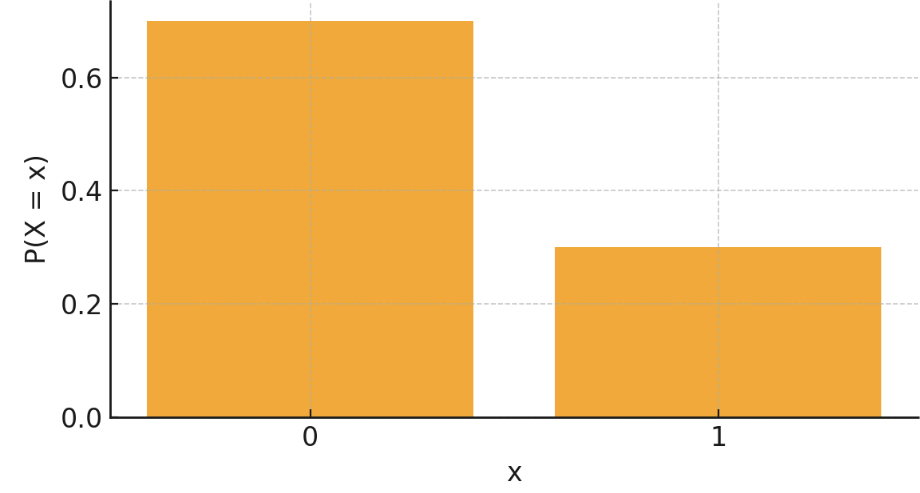
\includegraphics[width=0.6\textwidth]{figuras/dist_disc_bernoulli.png}
    \caption{Distribuição de Bernoulli.}
    \label{fig:dist_disc_bernoulli}
\end{figure}

\subsection{Distribuição Binomial}
O processo estocástico de Bernoulli possui as seguintes propriedades:
\begin{itemize}
    \item O experimento consiste de $n$ tentativas repetidas;
    \item Cada tentativa gera um resultado que pode ser classificado como sucesso ou falha;
    \item A probabilidade de sucesso $p$ se mantém constante de tentativa para tentativa;
    \item As tentativas são feitas de forma independente uma da outra.
\end{itemize}

Seja $X$ uma variável aleatória baseada em $n$ repetições de um processo de Bernoulli.  
Então a probabilidade de obtermos $k$ sucessos em $n$ repetições é dada por:
    $$
    P(X = k) = \binom{n}{k} p^k (1 - p)^{n - k}, \quad k = 0, 1, 2, \ldots, n
    $$,
onde:
    $$
    C_n^k = \binom{n}{k} = \frac{n!}{(n - k)! \, k!}
    $$
é uma combinação de $n$ elementos tomados de $k$ em $k$.

Então,
    $$
    E[X] = n \cdot p,
    $$
    $$
    V(X) = n \cdot p \cdot (1-p)
    $$

A Figura~\ref{fig:dist_disc_binomial} apresenta um exemplo de Distribuição Binomial.

\begin{figure}[H]
    \centering
    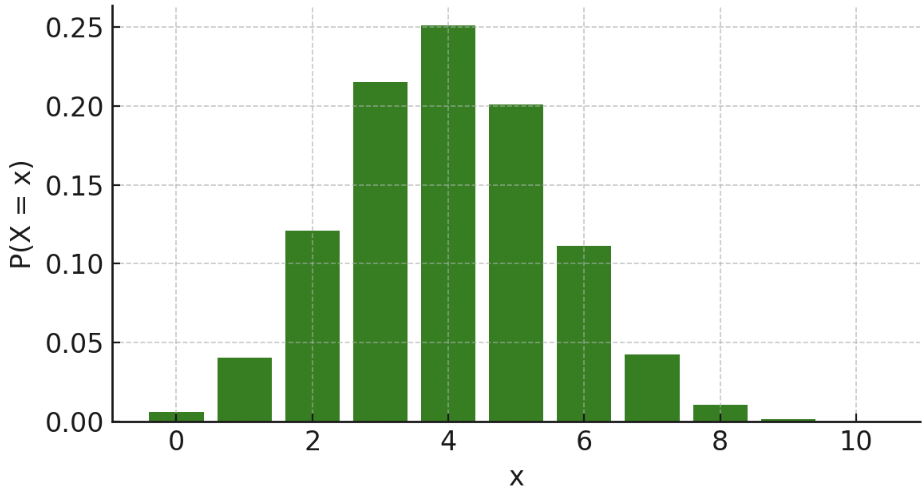
\includegraphics[width=0.6\textwidth]{figuras/dist_disc_binomial.png}
    \caption{Distribuição Binomial.}
    \label{fig:dist_disc_binomial}
\end{figure}

A seguir, apresentamos um exemplo de problema que pode ser modelado por meio da Distribuição Binomial:
\begin{quote}
``Uma urna tem 20 bolas pretas e 30 brancas. Retiram-se 25 bolas com reposição. Qual a probabilidade de que 2 sejam pretas?''
\end{quote}

\subsection{Distribuição de Poisson}
O processo estocástico de Poisson possui as seguintes propriedades:
\begin{itemize}
    \item O processo modela a ocorrência de eventos ao longo do tempo ou espaço contínuo;
    \item Existe uma taxa média constante $\lambda > 0$, que representa o número esperado de eventos por unidade de tempo (ou espaço);
    \item Os eventos ocorrem de forma independente em intervalos disjuntos;
    \item A probabilidade acumulada de ocorrência de eventos aumenta com o tempo.
\end{itemize}

Uma variável aleatória discreta $X$ segue o modelo de Poisson com taxa $\lambda > 0$ se:
    $$
    P(X = k) = \frac{e^{-\lambda} \lambda^k}{k!}, \quad k = 0, 1, 2, \ldots
    $$

Então,
    $$
    E[X] = \lambda,
    $$
    $$
    V(X) = \lambda
    $$

A Figura~\ref{fig:dist_disc_poisson} apresenta um exemplo de Distribuição de Poisson.

\begin{figure}[H]
    \centering
    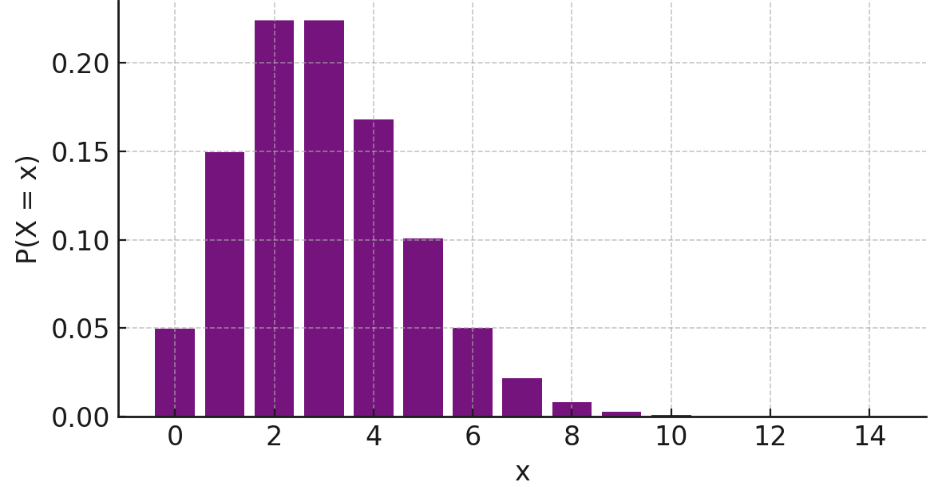
\includegraphics[width=0.6\textwidth]{figuras/dist_disc_poisson.png}
    \caption{Distribuição de Poisson.}
    \label{fig:dist_disc_poisson}
\end{figure}

A seguir, apresentamos um exemplo de problema que pode ser modelado por meio da Distribuição de Poisson:
\begin{quote}
``Numa estrada há 2 acidentes para cada 100 km. Qual a probabilidade de que em 250 km ocorram pelo menos 3 acidentes?''
\end{quote}

\subsection{Lei dos Eventos Raros}
Seja $X$ uma variável aleatória com Distribuição Binomial e $p$ a probabilidade de sucesso. Então,
    $$
    \lim_{n \to \infty} \binom{n}{k} p^k (1 - p)^{n - k} = \frac{e^{-\lambda} \lambda^k}{k!}, \quad k = 0, 1, 2, \ldots,
    $$
onde $\lambda = np$ é constante.

\subsection{Distribuição Geométrica}
A Distribuição Geométrica modela o número de tentativas necessárias até a ocorrência do primeiro sucesso em uma sequência de experimentos de Bernoulli independentes. Suas principais características são:

\begin{itemize}
    \item Cada tentativa resulta em um sucesso (com probabilidade $p$) ou uma falha (com probabilidade $1 - p$);
    \item As tentativas são independentes entre si;
    \item A variável aleatória $X$ representa o número de tentativas até o primeiro sucesso (inclusive o sucesso), ou, equivalentemente, o número de falhas antes do primeiro sucesso.
\end{itemize}

Dizemos que a variável aleatória discreta $X$ segue uma Distribuição Geométrica se:
    $$
    P(X = k) = p(1 - p)^{k - 1}, \quad k = 1, 2, \ldots
    $$

Então,
    $$
    E[X] = \frac{1}{p},
    $$
    $$
    V(X) = \frac{1 - p}{p^2}
    $$

A Figura~\ref{fig:dist_disc_geometrica} apresenta um exemplo de Distribuição Geométrica.

\begin{figure}[H]
    \centering
    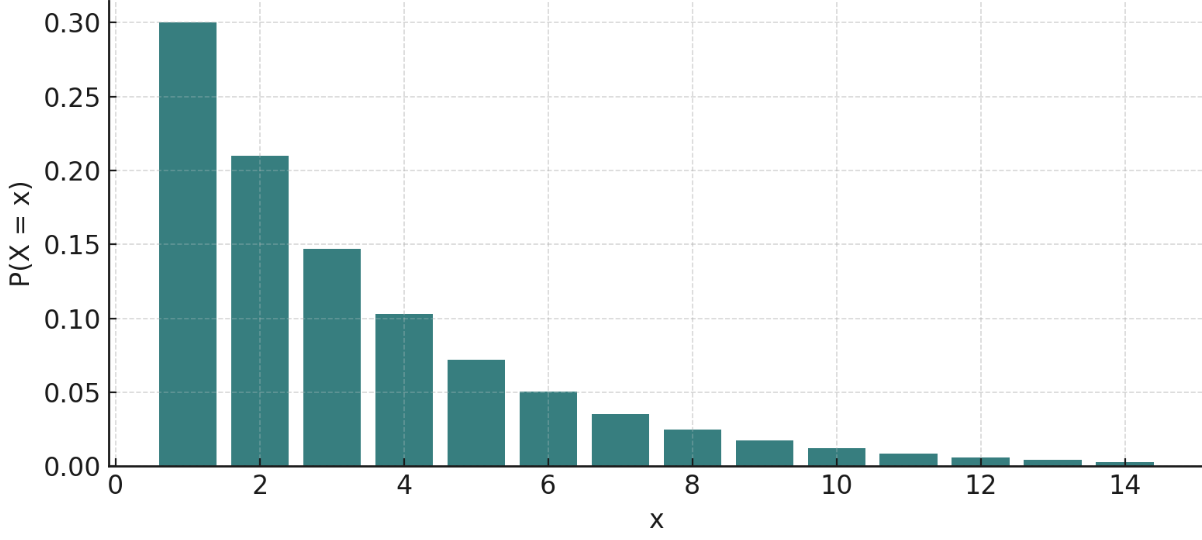
\includegraphics[width=0.75\textwidth]{figuras/dist_disc_geometrica.png}
    \caption{Distribuição Geométrica.}
    \label{fig:dist_disc_geometrica}
\end{figure}

A seguir, apresentamos um exemplo de problema que pode ser modelado por meio da Distribuição Geométrica:
\begin{quote}
``Suponha que temos uma urna com 36 bolas, sendo 27 bolas brancas e 9 pretas. Bolas são retiradas até que uma bola preta apareça. Qual é a probabilidade de que precisaremos de mais de 6 retiradas para sortear a primeira bola preta?''
\end{quote}

\subsection{Distribuição Binomial Negativa}
A Distribuição Binomial Negativa é apropriada para modelar situações em que se deseja saber a probabilidade de que um número fixo de sucessos ocorra na $k$-ésima tentativa, ou seja, quantas falhas ocorrem antes de alcançar um número pré-determinado de sucessos.
\begin{itemize}
    \item Os experimentos são independentes e possuem apenas dois resultados possíveis: sucesso ou falha;
    \item A probabilidade de sucesso $p$ é constante em cada tentativa;
    \item O processo continua até que um número fixo de sucessos seja alcançado.
\end{itemize}

Seja $X$ o número de repetições necessárias a fim de que ocorram exatamente $r$ sucessos, de modo que o $r$-ésimo sucesso ocorra na $k$-ésima tentativa. Então,
    $$
    P(X = k) = \binom{k - 1}{r - 1} p^r (1 - p)^{k - r}, \quad k = r, r + 1, \ldots
    $$

A Figura~\ref{fig:dist_disc_binomial_negativa} apresenta um exemplo de Distribuição Binomial Negativa.

\begin{figure}[H]
    \centering
    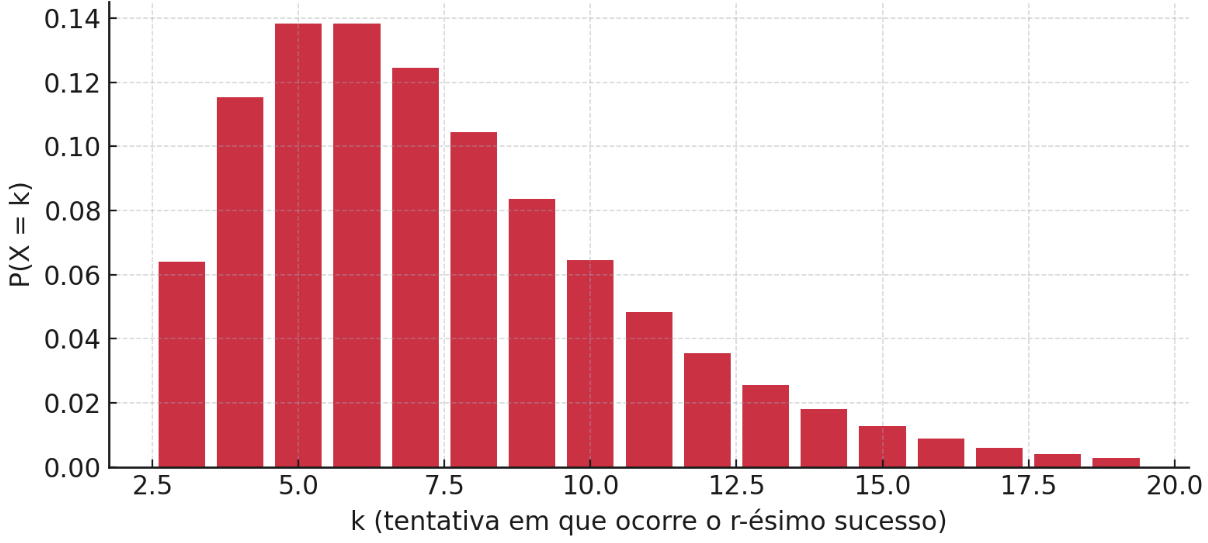
\includegraphics[width=0.75\textwidth]{figuras/dist_disc_binomial_negativa.png}
    \caption{Distribuição Binomial Negativa.}
    \label{fig:dist_disc_binomial_negativa}
\end{figure}

A seguir, apresentamos um exemplo de problema que pode ser modelado por meio da Distribuição Binomial Negativa:
\begin{quote}
``Em uma série da liga de futebol amador de uma cidade, o time que ganhar quatro jogos em sete será o vencedor. Suponha que o time
A tenha probabilidade $p = 0,6$ de ganhar do time B. Qual é a probabilidade de que A vença a série em seis jogos?''
\end{quote}

\subsection{Distribuição Hipergeométrica}
A Distribuição Hipergeométrica é semelhante à Distribuição Binomial, porém com uma diferença essencial: as retiradas são feitas sem reposição. Enquanto a Distribuição Binomial assume que cada tentativa é independente e a probabilidade de sucesso permanece constante (devido à reposição), a Distribuição Hipergeométrica modela situações em que a probabilidade de sucesso varia a cada retirada, pois os elementos não são devolvidos ao conjunto.

Considere um conjunto de $N$ objetos, dos quais $N_1$ são do tipo 1 e $N_2 = N - N_1$ são do tipo 2.  
Para um sorteio de $n$ objetos ($n < N$), sem reposição, seja $X$ a variável aleatória que define o número de objetos do tipo 1 sorteados.  
Então, a probabilidade de sortearmos $k$ objetos do tipo 1 é:
    $$
    P(X = k) = \frac{\binom{N_1}{k} \binom{N - N_1}{n - k}}{\binom{N}{n}}, \quad k = 0, 1, \ldots, n
    $$

A Figura~\ref{fig:dist_disc_hipergeometrica} apresenta um exemplo de Distribuição Hipergeométrica.

\begin{figure}[H]
    \centering
    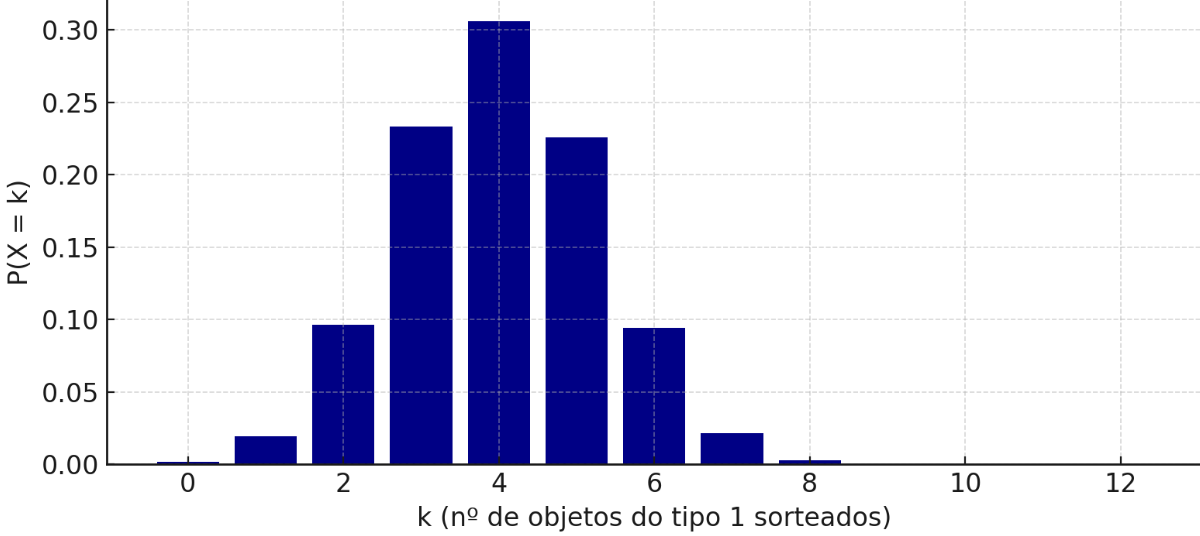
\includegraphics[width=0.75\textwidth]{figuras/dist_disc_hipergeometrica.png}
    \caption{Distribuição Hipergeométrica.}
    \label{fig:dist_disc_hipergeometrica}
\end{figure}

A seguir, apresentamos um exemplo de problema que pode ser modelado por meio da Distribuição Hipergeométrica:
\begin{quote}
``Numa urna há 40 bolas brancas e 60 pretas. Retiram-se 20 bolas. Qual a probabilidade de que ocorram no mínimo 2 bolas brancas, considerando extrações sem reposição?''
\end{quote}

\section{Modelos Probabilísticos Contínuos}

\subsection{Distribuição Uniforme Contínua}
Uma variável aleatória contínua $X$ segue uma Distribuição Uniforme se sua função densidade de probabilidade é dada por:
    $$
    f(x) = \begin{cases}
    \frac{1}{b - a}, & x \in [a, b] \\
    0, & x \notin [a, b]
    \end{cases}
    $$
Então,
    $$
    E[X] = \frac{a + b}{2},
    $$
    $$
    V(X) = \frac{(b - a)^2}{12}
    $$
A Figura~\ref{fig:dist_cont_uniforme} apresenta um exemplo de Distribuição Uniforme contínua.

\begin{figure}[H]
    \centering
    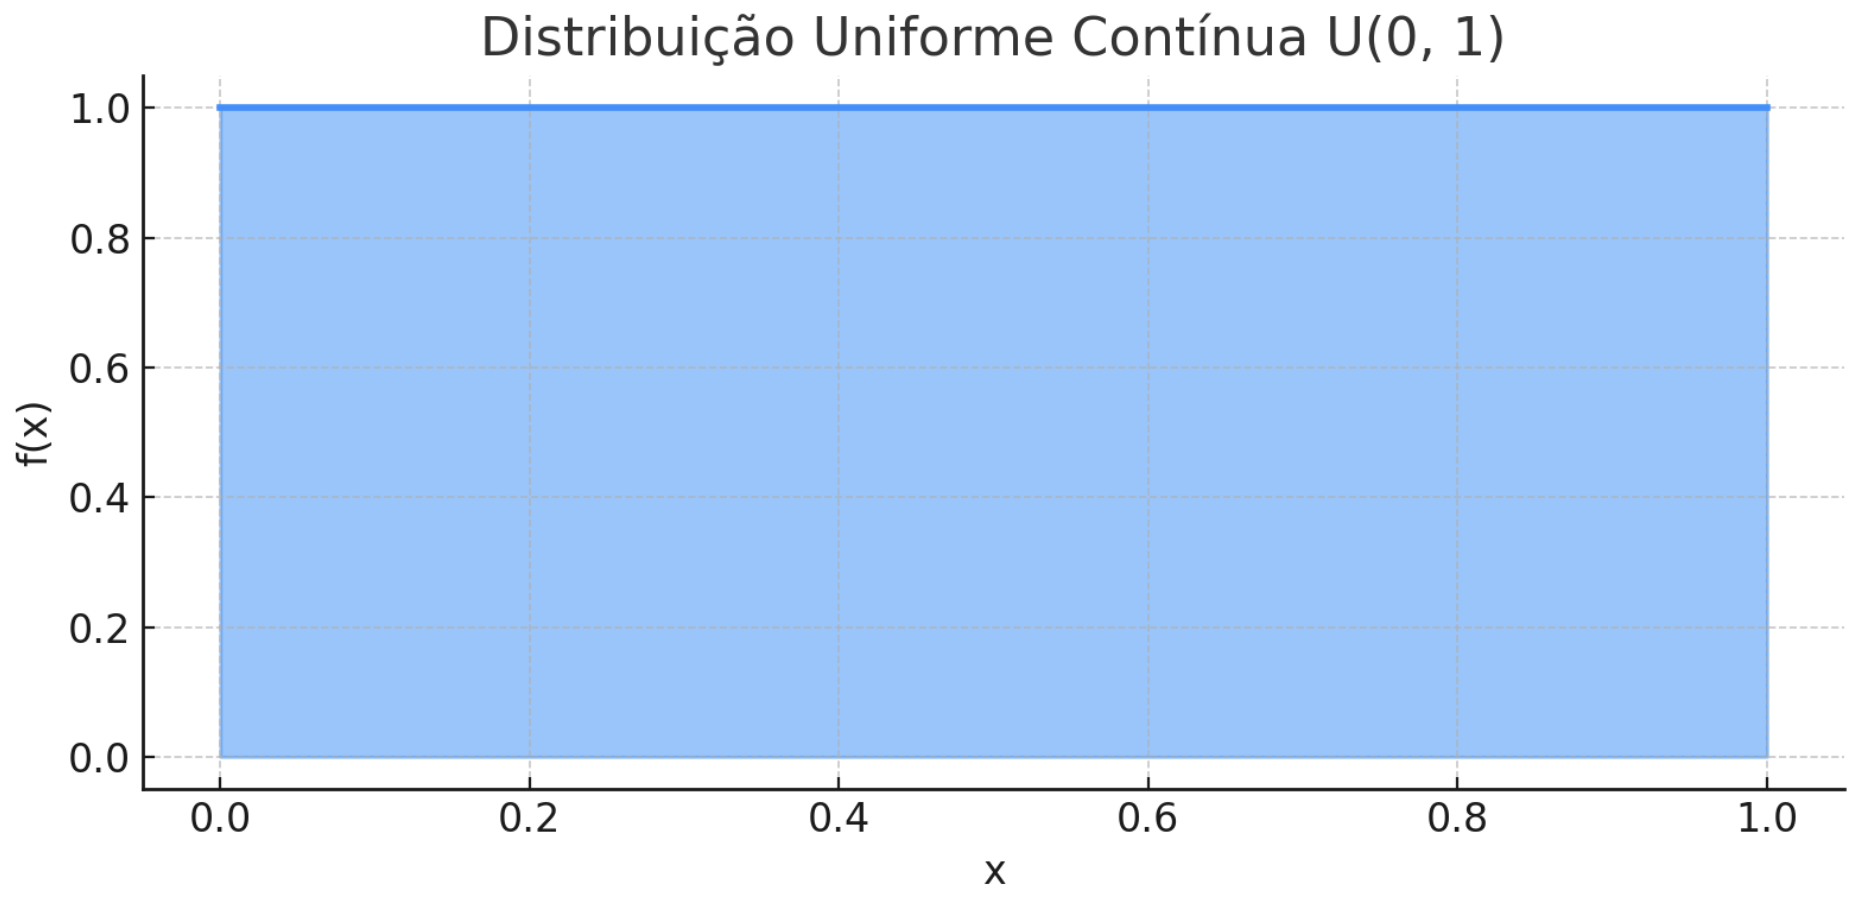
\includegraphics[width=0.6\textwidth]{figuras/dist_cont_uniforme.png}
    \caption{Distribuição Uniforme contínua.}
    \label{fig:dist_cont_uniforme}
\end{figure}

\subsection{Distribuição Normal}
Uma variável aleatória contínua $X$ que tome todos os valores na reta real segue a Distribuição Normal (ou Gaussiana) se sua função densidade de probabilidade é definida por:
    $$
    f(x) = \frac{1}{\sigma \sqrt{2\pi}} \exp\left[ -\frac{1}{2} \left( \frac{x - \mu}{\sigma} \right)^2 \right], \quad -\infty < x < \infty
    $$
onde $\mu = E[X]$ e $\sigma^2 = V(X) > 0$.


A Distribuição Normal apresenta as seguintes propriedades:
\begin{itemize}
    \item $f(x)$ é simétrica em relação à $\mu$.
    \item $f(x) \to 0$ quando $x \to \pm\infty$.
    \item O valor máximo de $f(x)$ ocorre em $x = \mu$.
\end{itemize}


Se $X$ é uma variável aleatória contínua com Distribuição Normal, $X \sim \mathcal{N}(\mu, \sigma^2)$, e se $Y = aX + b$, com $a$ e $b$ constantes, então
    $$
    Y \sim \mathcal{N}(a\mu + b, a^2\sigma^2).
    $$
Seja $X \sim \mathcal{N}(\mu, \sigma^2)$. Se
    $$
    Z = \frac{X - \mu}{\sigma},
    $$
então $Z \sim \mathcal{N}(0, 1)$.

Assim,
\begin{align*}
    P(a \leq X \leq b) &= P\left( \frac{a - \mu}{\sigma} \leq \frac{X - \mu}{\sigma} \leq \frac{b - \mu}{\sigma} \right) \\
    &= P\left( \frac{a - \mu}{\sigma} \leq Z \leq \frac{b - \mu}{\sigma} \right) \\
    &= P(X \leq b) - P(X \leq a).
\end{align*}

A tabela Normal pode ser acessada através do link \url{https://en.wikipedia.org/wiki/Standard_normal_table#Table_examples}.

A Figura~\ref{fig:dist_cont_normal} apresenta um exemplo de Distribuição Normal. Note que $\mu$ define o centro da curva e $\sigma$ a abertura.

\begin{figure}[H]
    \centering    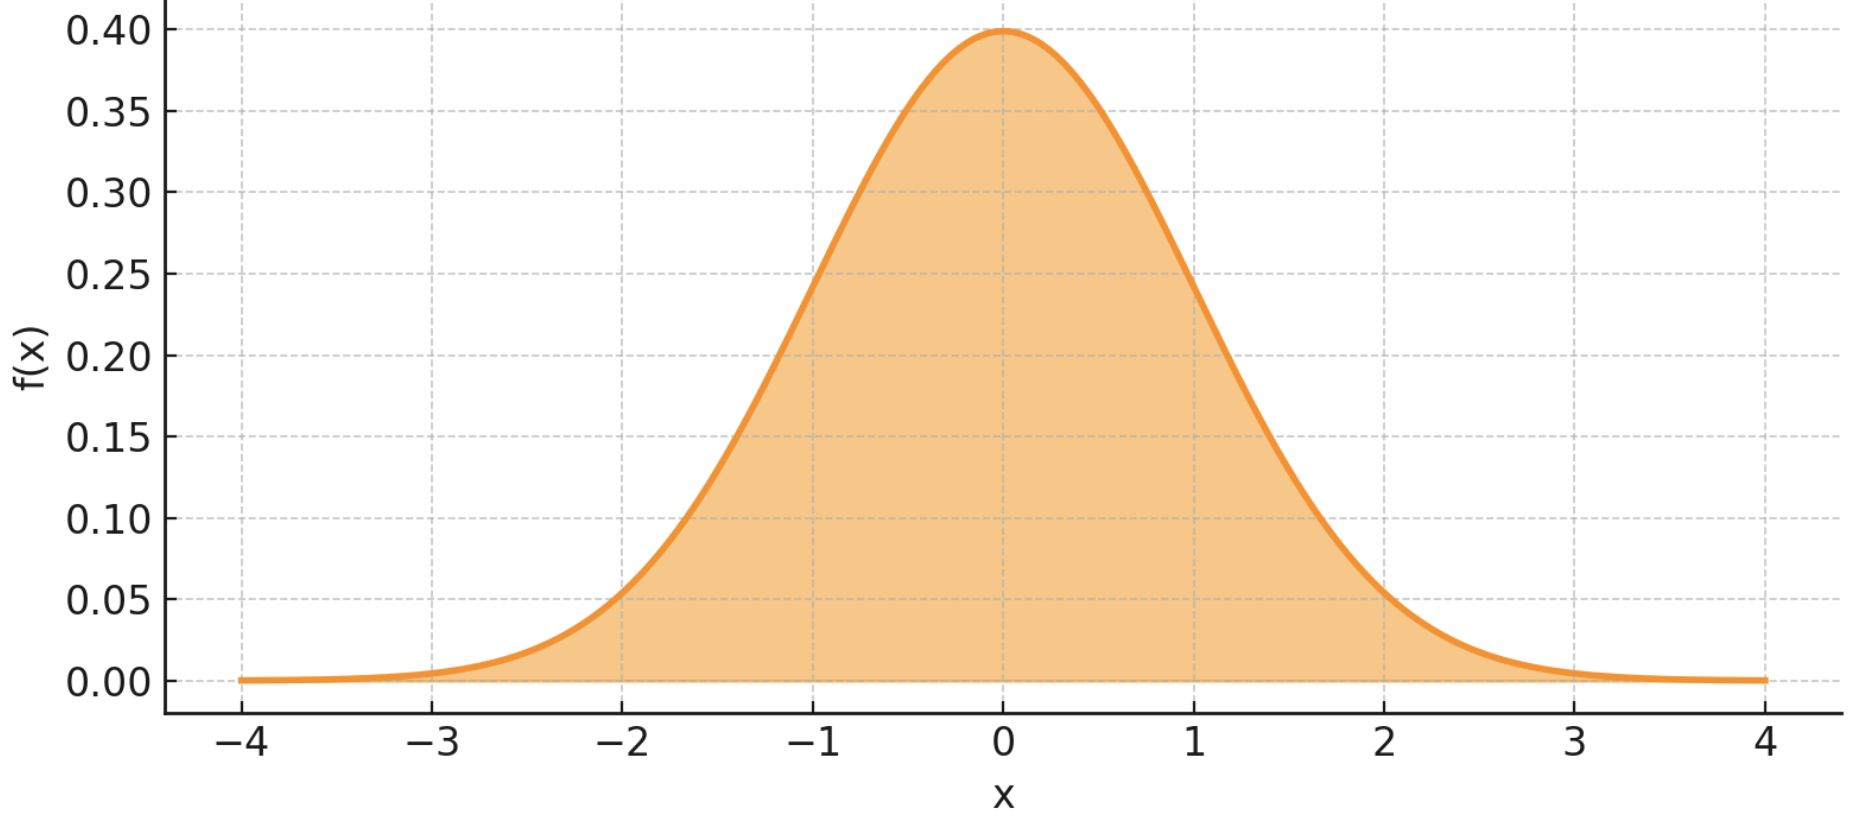
\includegraphics[width=0.75\textwidth]{figuras/dist_cont_normal.png}
    \caption{Distribuição Normal.}
    \label{fig:dist_cont_normal}
\end{figure}

\subsection{Distribuição Exponencial}
Uma variável aleatória contínua $X$ segue o modelo exponencial se sua função densidade de probabilidade é dada por:
    $$
    f(x) = 
    \begin{cases}
    \lambda e^{-\lambda x}, & x \geq 0 \\
    0, & x < 0
    \end{cases}
    $$
onde $\lambda > 0$ e $-\infty < x < \infty$.

Então,
    $$
    E[X] = \frac{1}{\lambda},
    $$
    $$
    V(X) = \frac{1}{\lambda^2}
    $$

E a função de distribuição acumulada é dada por:
    $$
    F(x) = 
    \begin{cases}
    1 - e^{-\lambda x}, & x \geq 0 \\
    0, & x < 0
    \end{cases}
    $$

A Distribuição Exponencial é derivada a partir de um processo de Poisson (cadeia de Markov de tempo contínuo). Ela apresenta a propriedade de ``ausência de memória'', isto é:
    $$
    P(X \geq t + s \mid X \geq s) = P(X \geq t)
    $$

A Figura~\ref{fig:dist_cont_exponencial} apresenta um exemplo de Distribuição Exponencial. Note que $\lambda$ é onde começa o decaimento no eixo y.

\begin{figure}[H]
    \centering    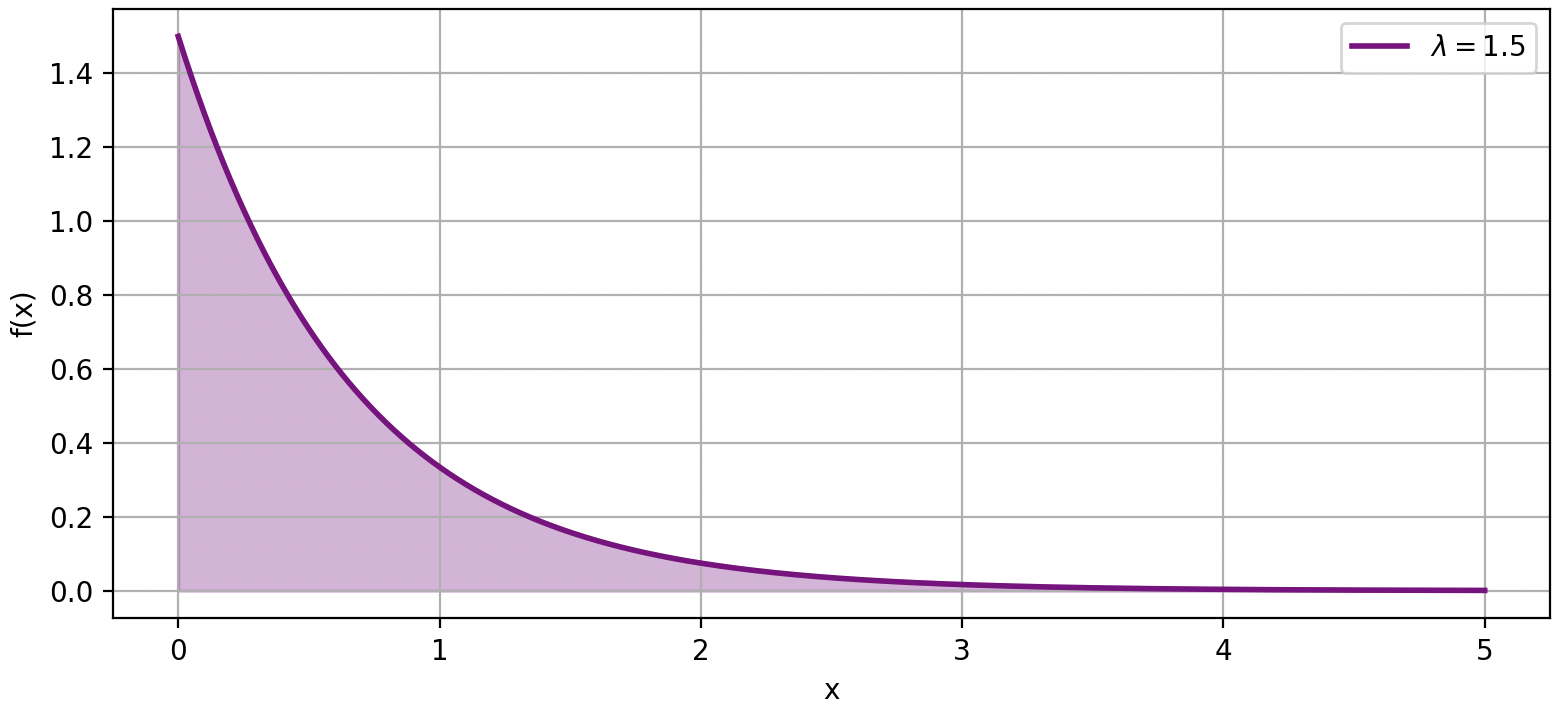
\includegraphics[width=0.75\textwidth]{figuras/dist_cont_exponencial.png}
    \caption{Distribuição Exponencial.}
    \label{fig:dist_cont_exponencial}
\end{figure}

\subsection{Distribuição Gama}
Uma variável aleatória contínua $X$ tem Distribuição Gama com parâmetros $\lambda > 0$ e $\alpha > 0$, se sua função densidade de probabilidade é dada por:
    $$
    f(x) =
    \begin{cases}
    \frac{\lambda^\alpha}{\Gamma(\alpha)} x^{\alpha - 1} e^{-\lambda x}, & x \geq 0, \\
    0, & x < 0,
    \end{cases}
    $$
onde $\Gamma$ é a função gama:
    $$
    \Gamma(\alpha) = \int_0^{\infty} t^{\alpha - 1} e^{-t} \, dt.
    $$

Então,
    $$
    E[X] = \frac{\alpha}{\lambda},
    $$
    $$
    V(X) = \frac{\alpha}{\lambda^2}
    $$

Se $\alpha$ for um número inteiro positivo, a distribuição representará uma Distribuição Erlang, ou seja, a soma de $\alpha$ variáveis aleatórias independentes distribuídas exponencialmente, cada uma delas com uma média $\theta = 1/\lambda$.

A Distribuição Exponencial é um caso especial da Distribuição Gama onde $\alpha = 1$.

A Figura~\ref{fig:dist_cont_gama} apresenta um exemplo de Distribuição Gama.

\begin{figure}[H]
    \centering    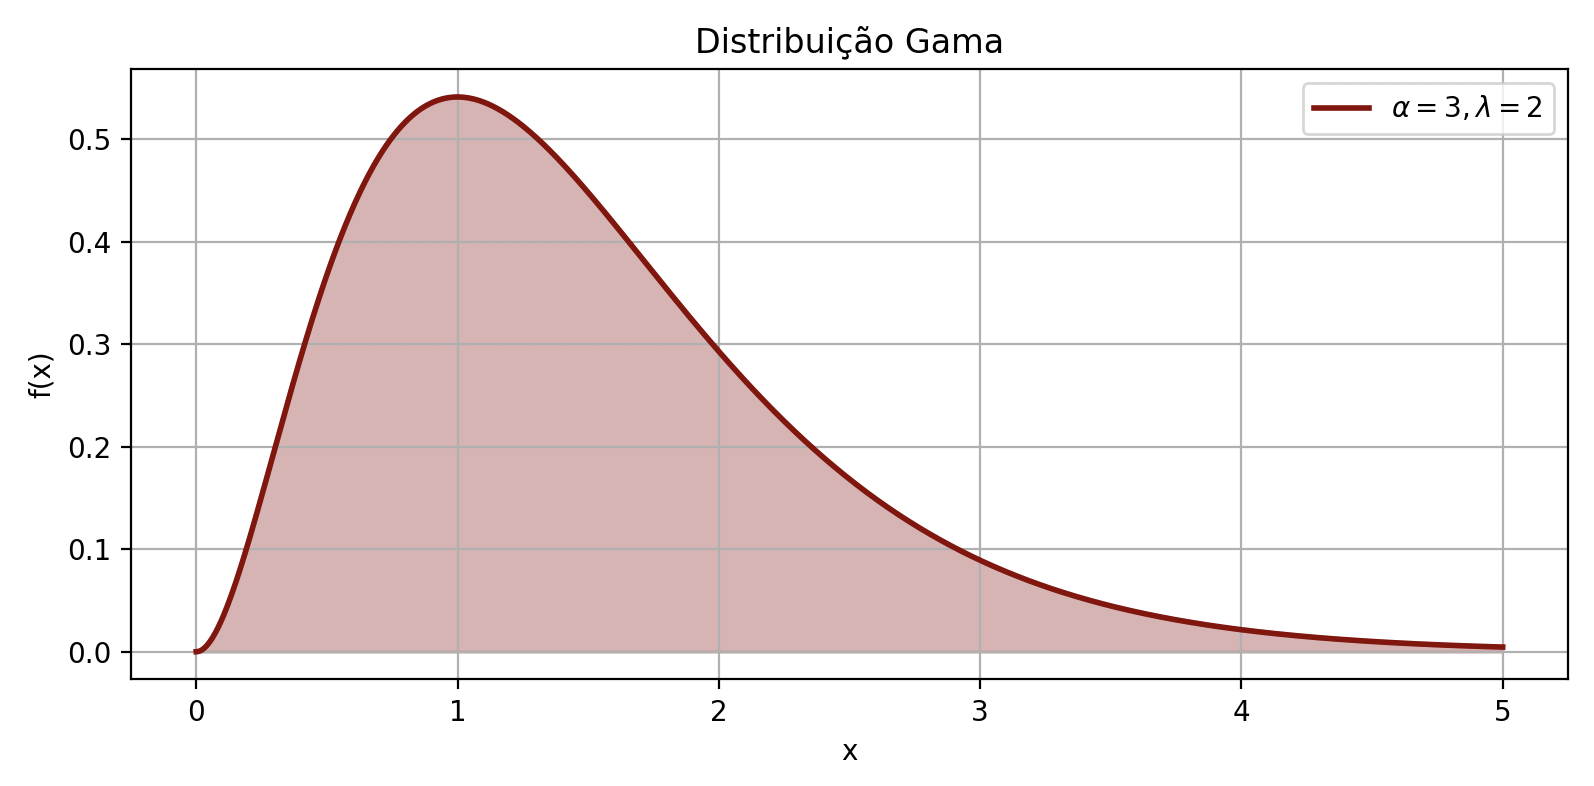
\includegraphics[width=0.75\textwidth]{figuras/dist_cont_gama.png}
    \caption{Distribuição Gama.}
    \label{fig:dist_cont_gama}
\end{figure}

\subsection{Distribuição Qui-Quadrado}
A variável aleatória contínua $X$ segue a Distribuição Qui-Quadrado (denominada $\chi^2$) se sua função densidade de probabilidade é dada por:
    $$
    f(x) = 
    \begin{cases}
    \frac{x^{k/2 - 1} e^{-x/2}}{2^{k/2} \Gamma(k/2)}, & x > 0, \\
    0, & x \leq 0,
    \end{cases}
    $$

A Distribuição Qui-Quadrado é definida pela soma de $k$ distribuições normais padronizadas e independentes. Ou seja, $X$ tem Distribuição Qui-Quadrado com $k$ graus de liberdade se
    $$
    X = \sum_{i=1}^{k} Z_i^2,
    $$
onde $Z_1, Z_2, \ldots, Z_k$ são variáveis aleatórias com Distribuição Normal padronizada,
    $$
    Z_i \sim \mathcal{N}(\mu = 0, \sigma^2 = 1), \quad i = 1, \ldots, k.
    $$

Para denominar que $X$ segue uma Distribuição Qui-Quadrado, usamos $X \sim \chi^2(k)$ ou $X \sim \chi_k^2$.

A Figura~\ref{fig:dist_cont_quiquadrado} apresenta um exemplo de Distribuição Qui-Quadrado.

\begin{figure}[H]
    \centering    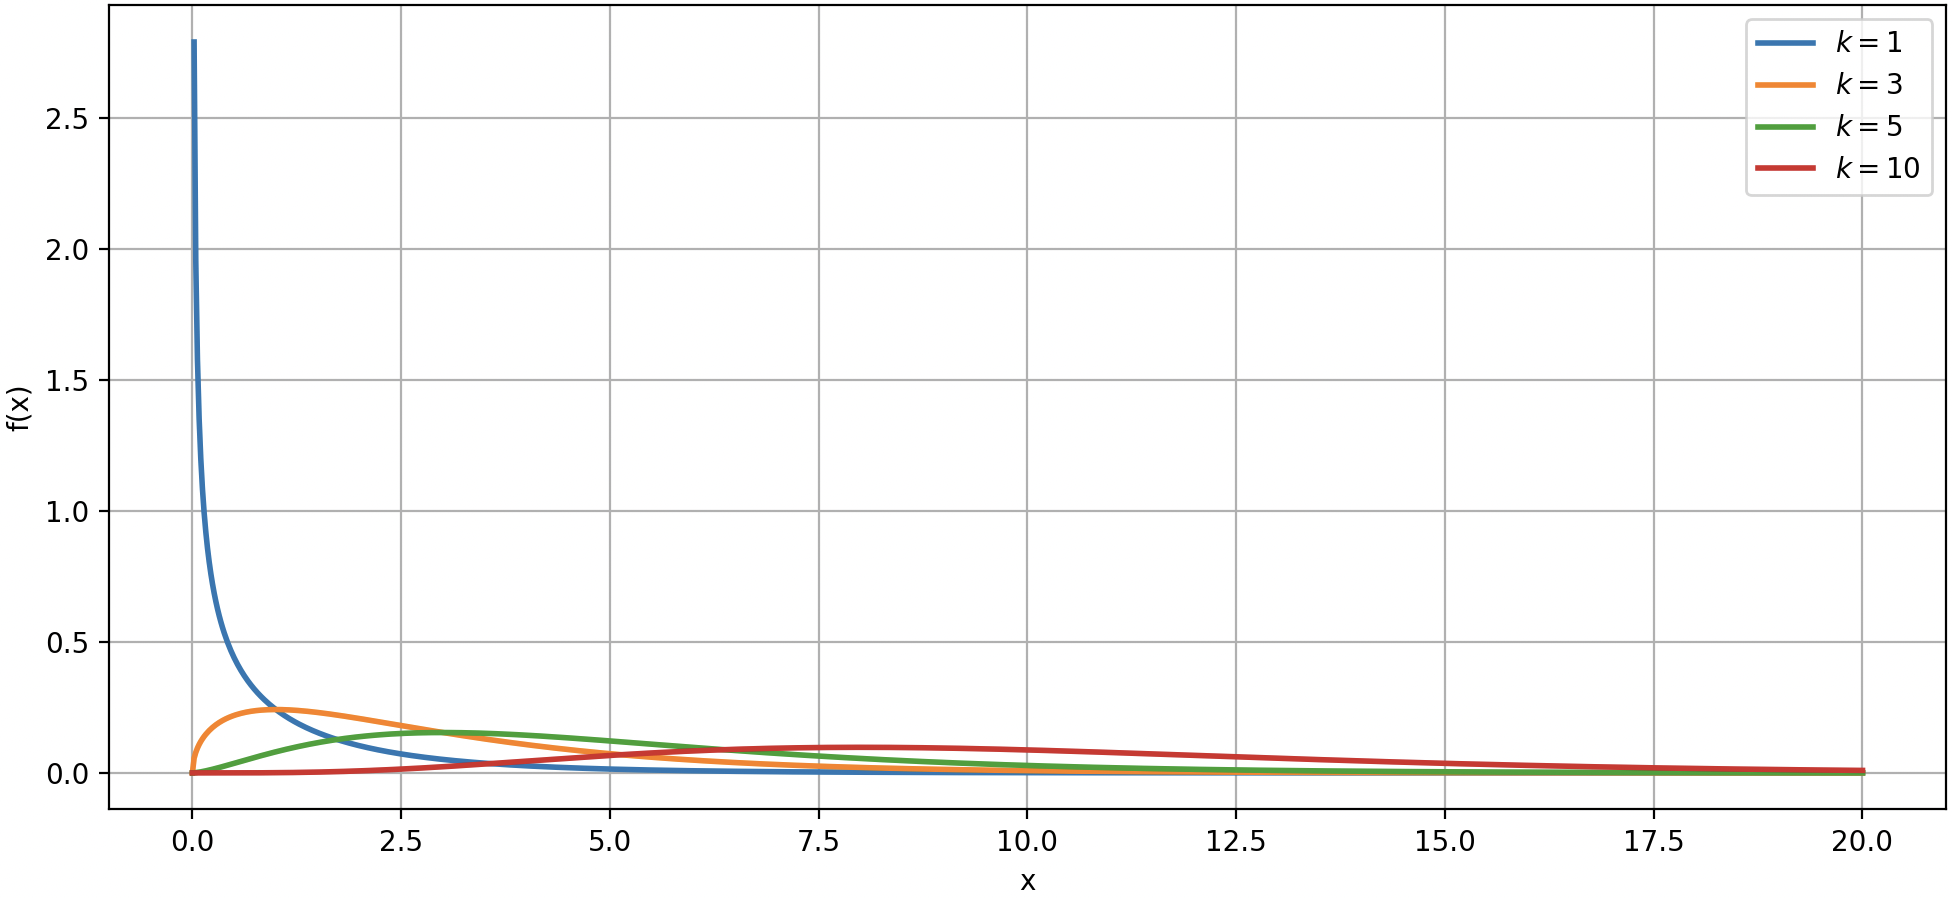
\includegraphics[width=0.75\textwidth]{figuras/dist_cont_quiquadrado.png}
    \caption{Distribuição Qui-Quadrado.}
    \label{fig:dist_cont_quiquadrado}
\end{figure}

\subsection{Distribuição Beta}
Seja $X$ uma variável aleatória contínua limitada em $[0,1]$. Dizemos que $X$ segue uma Distribuição Beta se sua função densidade de probabilidade é dada por:
    $$
    f(x) =
    \begin{cases}
    \frac{1}{B(\alpha, \beta)} x^{\alpha - 1} (1 - x)^{\beta - 1}, & 0 < x < 1, \\
    0, & \text{caso contrário},
    \end{cases}
    $$
onde $\alpha, \beta > 0$ e
    $$
    B(\alpha, \beta) = \int_0^1 x^{\alpha - 1} (1 - u)^{\beta - 1} \, du,
    $$
é a função beta, que atua como uma constante de normalização para que a área da função densidade de probabilidade seja igual a um.

A Figura~\ref{fig:dist_cont_beta} apresenta um exemplo de Distribuição Beta. Note que o limite onde ela é definida no eixo x é de 0 a 1.

\begin{figure}[H]
    \centering    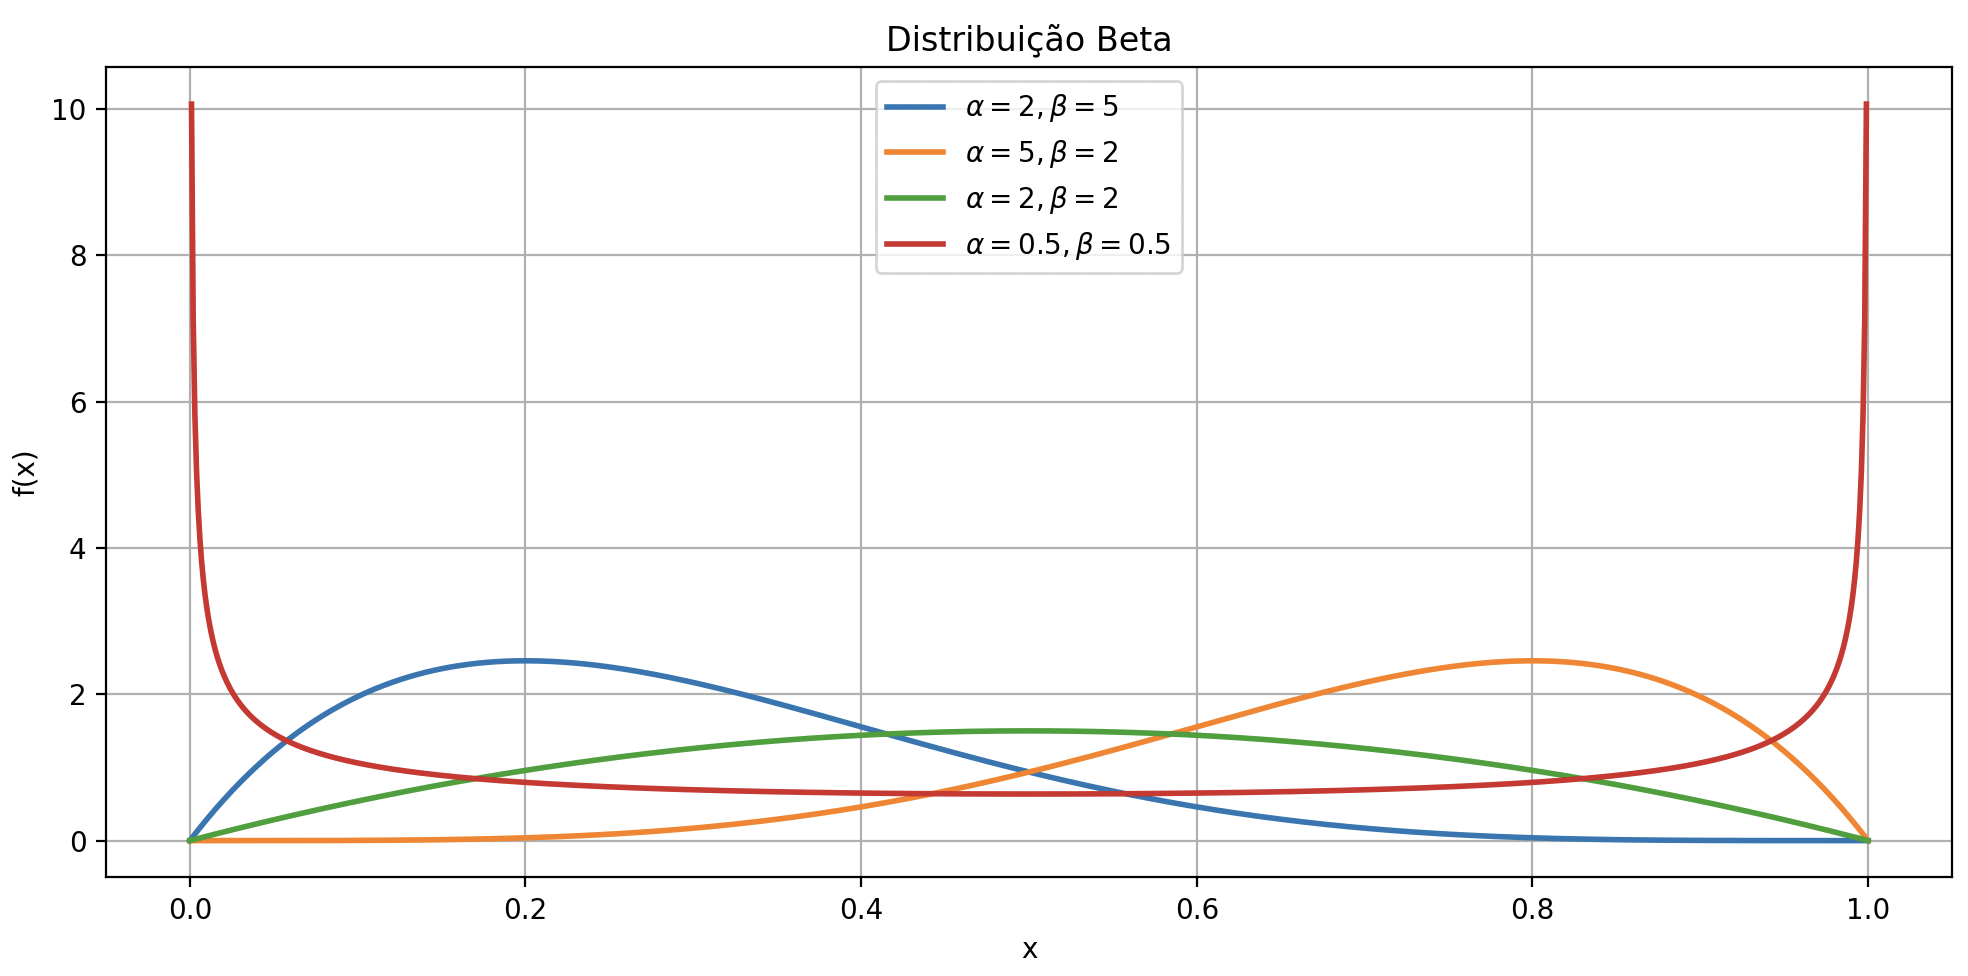
\includegraphics[width=0.75\textwidth]{figuras/dist_cont_beta.png}
    \caption{Distribuição Beta.}
    \label{fig:dist_cont_beta}
\end{figure}

\subsection{Distribuição t de Student}
A variável aleatória $X$ tem Distribuição t de Student com $\nu$ graus de liberdade se sua função densidade de probabilidade é dada por:
    $$
    f(x) = \frac{\Gamma\left(\frac{\nu+1}{2}\right)}{\sqrt{\nu \pi} \, \Gamma\left(\frac{\nu}{2}\right)} \left(1 + \frac{x^2}{\nu} \right)^{-\frac{\nu+1}{2}}, \quad -\infty < x < \infty
    $$
onde $\Gamma$ é a função gama:
    $$
    \Gamma(\alpha) = \int_0^{\infty} t^{\alpha - 1} e^{-t} \, dt
    $$

Quando aumentamos $\nu$, a distribuição se aproxima da Distribuição Normal.

A Figura~\ref{fig:dist_cont_tstudent} apresenta um exemplo de Distribuição t de Student.

\begin{figure}[H]
    \centering    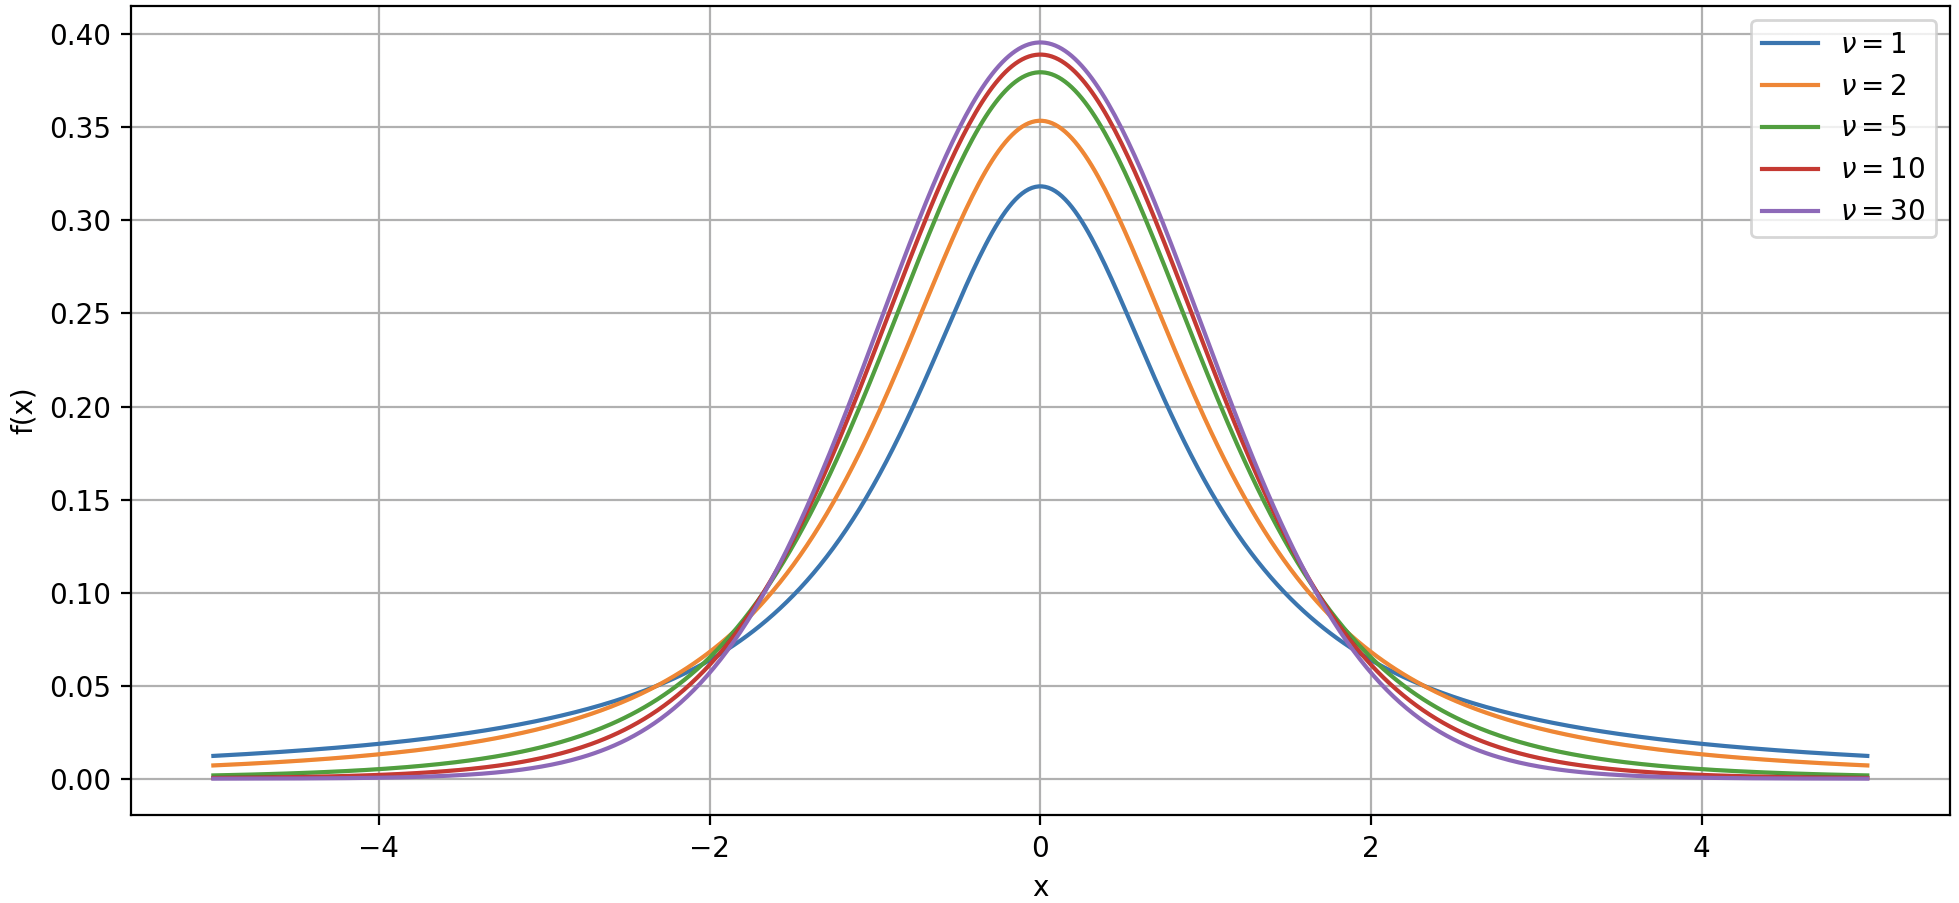
\includegraphics[width=0.75\textwidth]{figuras/dist_cont_tstudent.png}
    \caption{Distribuição t de Student.}
    \label{fig:dist_cont_tstudent}
\end{figure}

\subsection{Distribuição Weibull}

Dizemos que a variável aleatória contínua $X$ segue a Distribuição Weibull se:
    $$
    f(x; \lambda, k) =
    \begin{cases}
    \frac{k}{\lambda} \left( \frac{x}{\lambda} \right)^{k-1} e^{-(x/\lambda)^k}, & x \ge 0, \\
    0, & x < 0,
    \end{cases}
    $$

Então,
    $$
    E[X] = \lambda \, \Gamma\left(1 + \frac{1}{k}\right),
    $$
    $$
    \mathrm{var}[X] = \lambda^2 \left[ \Gamma\left( 1 + \frac{2}{k} \right) - \left( \Gamma\left( 1 + \frac{1}{k} \right) \right)^2 \right]
    $$

A Distribuição Exponencial é um caso especial da Distribuição de Weibull onde $k = 1$.

A Figura~\ref{fig:dist_cont_weibull} apresenta um exemplo de Distribuição Weibull.

\begin{figure}[H]
    \centering    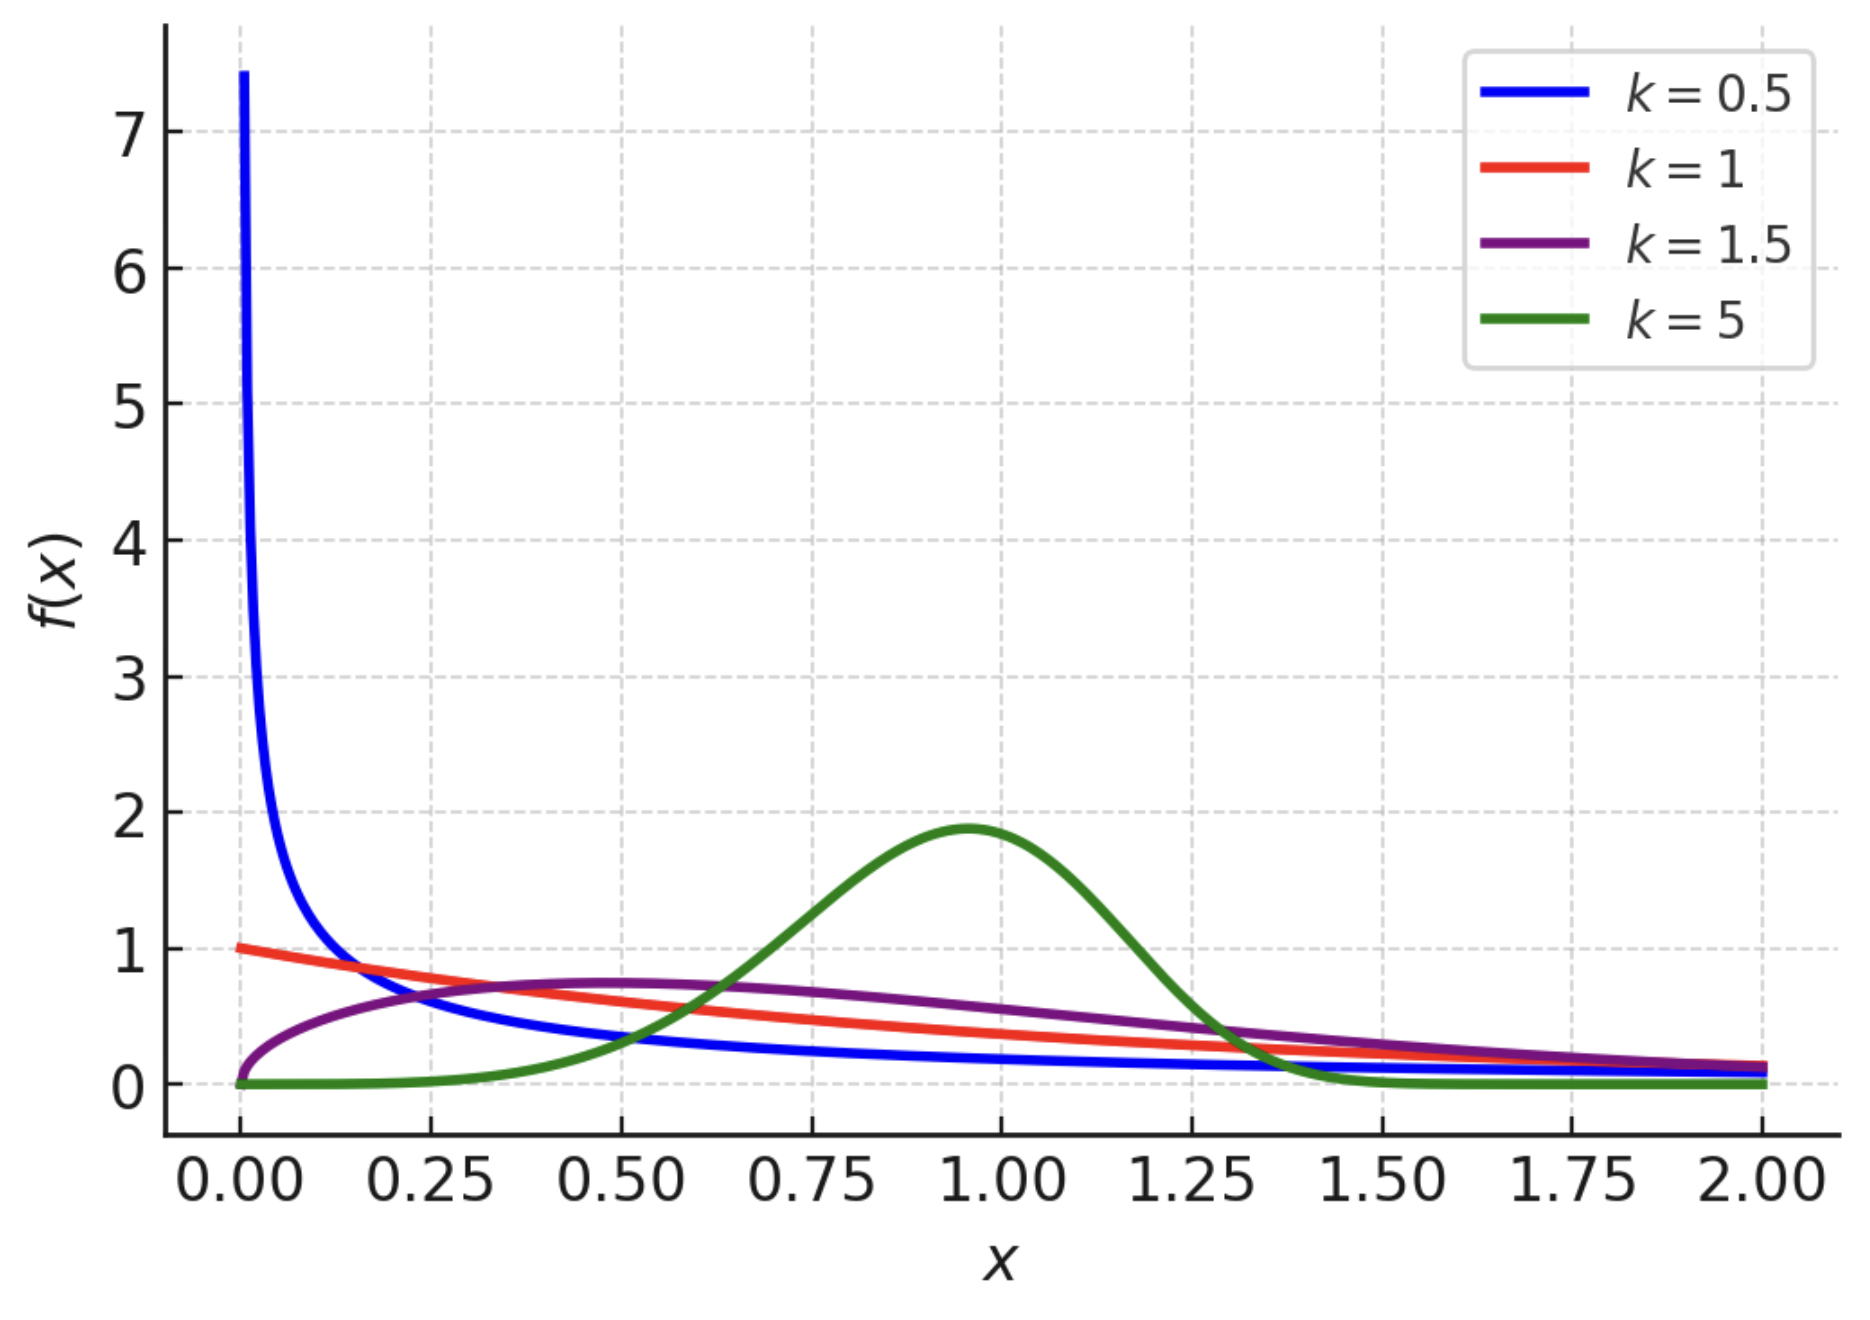
\includegraphics[width=0.6\textwidth]{figuras/dist_cont_weibull.png}
    \caption{Distribuição Weibull.}
    \label{fig:dist_cont_weibull}
\end{figure}

\section{Variáveis Aleatórias Multidimensionais}
\subsection{Discretas}
Seja $\epsilon$ um experimento aleatório associado a um espaço amostral $\Omega$. Sejam $X_1 = X_1(\omega), X_2 = X_2(\omega), \ldots$, funções que associam um número real a cada resultado $\omega \in \Omega$. 
Denominamos vetor aleatório o conjunto $\mathbf{X} = [X_1, X_2, \ldots]$.

Sejam $X$ e $Y$ variáveis aleatórias associadas a um espaço amostral $\Omega$. O par $(X, Y)$ será uma variável aleatória discreta bidimensional se os valores possíveis forem finitos ou infinitos enumeráveis.  A cada resultado possível $(x_i, y_j)$, $i, j = 1, 2, \ldots$, associamos um número
    $$
    p(x_i, y_j) = P(X = x_i, Y = y_j)
    $$
satisfazendo:
\begin{itemize}
    \item $0 \leq P(X = x_i, Y = y_j) \leq 1 \quad \forall\,(x_i, y_j),\ i, j = 1, 2, \ldots$
    \item $\displaystyle \sum_{i=1}^{\infty} \sum_{j=1}^{\infty} P(X = x_i, Y = y_j) = 1$
\end{itemize}

\subsection{Contínuas}
Sejam $X$ e $Y$ variáveis aleatórias associadas a um espaço amostral $\Omega$. O par $(X, Y)$ será uma variável aleatória contínua bidimensional se $(X, Y)$ tomar todos os valores em algum conjunto não enumerável do $\mathbb{R}^2$. A esse par, associamos uma função densidade de probabilidade conjunta que satisfaz:

\begin{itemize}
    \item $f(x, y) \geq 0 \quad \forall (x, y) \in \mathbb{R}^2$
    \item $\displaystyle \int_{-\infty}^{\infty} \int_{-\infty}^{\infty} f(x, y) \, dx \, dy = 1$
\end{itemize}

\subsection{Distribuição de Probabilidade Marginal}
Seja $(X, Y)$ uma variável aleatória discreta bidimensional.  
Então, a distribuição de probabilidade marginal de $X$ é definida por:
\begin{equation}
    P(X = x_i) = \sum_{j=1}^{\infty} P(X = x_i, Y = y_j)
\end{equation}
e a de $Y$:
\begin{equation}
    P(Y = y_j) = \sum_{i=1}^{\infty} P(X = x_i, Y = y_j)
\end{equation}

Então a função de densidade de probabilidade marginal é dada por:
As funções densidade de probabilidade marginais são dadas por:
    $$
    f_X(x) = \int_{-\infty}^{\infty} f(x, y) \, dy
    $$
    $$
    f_Y(y) = \int_{-\infty}^{\infty} f(x, y) \, dx
    $$

Então:
    $$
    P(a \leq x \leq b) = \int_a^b f_X(x) \, dx
    $$
    $$
    P(c \leq y \leq d) = \int_c^d f_Y(y) \, dy
    $$

\subsection{Probabilidade Condicional Discreta}
Seja o vetor aleatório bidimensional $(X, Y)$. A probabilidade condicional de $X = x$ dado que $Y = y$ foi observada é dada por:
    $$
    P(X = x \mid Y = y) = \frac{P(X = x, \, Y = y)}{P(Y = y)}, \quad P(Y = y) > 0.
    $$

\subsection{Probabilidade Condicional Contínua}
Seja $(X, Y)$ um vetor aleatório bidimensional contínuo com função densidade de probabilidade conjunta $f(x, y)$. 
Sejam $f_X(x)$ e $f_Y(y)$ as funções densidade de probabilidade marginais de $X$ e $Y$, respectivamente. 
Então, a função densidade de probabilidade condicional de $X$ dado que $Y = y$ é definida por:
    $$
    f_{X|Y}(x|y) = \frac{f(x, y)}{f_Y(y)}, \quad f_Y(y) > 0
    $$
e a função densidade de probabilidade condicional de $Y$ dado que $X = x$,
    $$
    f_{Y|X}(y|x) = \frac{f(x, y)}{f_X(x)}, \quad f_X(x) > 0
    $$

\subsection{Independência}
Dizemos que as variáveis aleatórias $X$ e $Y$ são independentes se, e somente se:

\begin{itemize}
    \item Caso discreto:
    $$
    P(X = x_i, Y = y_j) = P(X = x_i) P(Y = y_j), \quad \forall i \neq j
    $$
    \item Caso contínuo:
    $$
    f(x, y) = f_X(x) f_Y(y), \quad \forall (x, y) \in \mathbb{R}^2.
    $$
\end{itemize}

\section{Esperança Multidimensional}
Sejam $X$ e $Y$ variáveis aleatórias e $g(X,Y)$ uma função de $X$ e $Y$.
Então, a esperança de $g(X,Y)$ é definida por:

\begin{itemize}
    \item Caso discreto:
        $$
        E[g(X,Y)]
        = \sum_{i=1}^{\infty} \sum_{j=1}^{\infty}
        g(x_i, y_j)\, \Pr(X = x_i,\, Y = y_j)
        $$
    \item Caso contínuo:
        $$
        E[g(X,Y)]
        = \int_{-\infty}^{\infty}\!\!\int_{-\infty}^{\infty}
        g(x,y)\, f_{X,Y}(x,y)\, dx\, dy
        $$
\end{itemize}

Se as variáveis aleatórias $X$ e $Y$ forem independentes, então:
    $$
    E[XY] = E[X] \, E[Y]
    $$

\section{Variância Multidimensional}
Sejam $X$ e $Y$ variáveis aleatórias e $g(X,Y)$ uma função de $X$ e $Y$.
Então, a variância de $g(X,Y)$ é definida por:
    $$
    V[g(X,Y)] = E\left[ g(X,Y)^2 \right] - \left( E[g(X,Y)] \right)^2
    $$

Se as variáveis aleatórias $X$ e $Y$ forem independentes, então:
    $$
    V(X + Y) = V(X) + V(Y)
    $$

\section{Esperança Condicional}
A esperança condicional para as variáveis aleatórias $X$ e $Y$ é definida por:

\begin{itemize}
    \item Caso discreto:
        $$
        E[X \mid Y = y] = \sum_{i=1}^{n} x_i \, P(X = x_i \mid Y = y)
        $$
        $$
        E[Y \mid X = x] = \sum_{j=1}^{m} y_j \, P(Y = y_j \mid X = x)
        $$
    \item Caso contínuo:
        $$
        E[X \mid Y = y] = \int_{-\infty}^{\infty} x \, f_{X\mid Y}(x \mid y) \, dx
        $$
        $$
        E[Y \mid X = x] = \int_{-\infty}^{\infty} y \, f_{Y\mid X}(y \mid x) \, dy
        $$
\end{itemize}

\section{Variância Condicional}
A variância condicional para as variáveis aleatórias $X$ e $Y$ é definida por:
    $$
    V(X \mid Y) = E[X^2 \mid Y] - \{ E[X \mid Y] \}^2
    $$

\section{Lei da Esperança Total}
Sejam $X$ e $Y$ duas variáveis aleatórias. Então:
    $$
    E(X) = E\left[ E(X \mid Y) \right]
    $$

Assim, 
    $$
    E[X] = \sum_{y} E[X \mid Y = y] \, P(Y = y),
    $$
    $$
    E[Y] = \sum_{x} E[Y \mid X = x] \, P(X = x).
    $$

\section{Covariância}
Sejam $X$ e $Y$ variáveis aleatórias. A covariância de $X$ e $Y$ é definida por:
    $$
    \mathrm{Cov}(X, Y) = E\left[(X - E\left[X\right])(Y - E\left[Y\right])\right]
    $$
Portanto,
    $$
    \mathrm{Cov}(X, Y) = E\left[XY\right] - E\left[X\right]E(Y)
    $$

Note que:
    $$
    \mathrm{Cov}(X, X) = E\left[(X - E\left[X\right])^2\right] = V(X)
    $$

\section{Correlação de Pearson}
\label{sec:correlacao_pearson}
Sejam $X$ e $Y$ duas variáveis aleatórias. A correlação de $X$ e $Y$ é definida por:
    $$
    \rho_{X,Y} =
    \frac{E[(X - E[X])(Y - E[Y])]}{\sqrt{V(X)V(Y)}} =
    \frac{\mathrm{cov}(X, Y)}{\sigma_X \sigma_Y}
    $$
onde $V(X)$ e $V(Y)$ são as variâncias de $X$ e $Y$, respectivamente.

A correlação de Pearson nada mais é que a covariância normalizada (limitada entre -1 e 1).

O coeficiente de Pearson pode ser definido para uma amostra de dados, onde, nesse caso, usamos os estimadores da covariância e variância.
Assim, o coeficiente de Pearson para uma amostra é dado por:
    $$
    r = \frac{\sum_{i=1}^{n} (x_i - \bar{x})(y_i - \bar{y})}
    {\sqrt{\sum_{i=1}^{n} (x_i - \bar{x})^2} \, \sqrt{\sum_{i=1}^{n} (y_i - \bar{y})^2}},
    $$
onde $-1 \leq r \leq 1$ e $x_i, y_i$, $i = 1, 2, \ldots, n$, são os valores observados.

Quando a correlação de Pearson é igual a 0, não implica que não tem uma correlação, mas sim que essa correlação não é linear.

\section{Modelos Probabilísticos Multidimensionais}
\subsection{Distribuição Normal Multidimensional}

O vetor aleatório $\mathbf{X}$ segue a Distribuição Normal multidimensional se sua função densidade de probabilidade conjunta é dada por:
    $$
    f(x; \mu, \Sigma) =
    \frac{1}{\sqrt{(2\pi)^{d/2}|\Sigma|^{1/2}}}
    \exp\left( -\frac{1}{2}(x - \mu)^\top \Sigma^{-1} (x - \mu) \right),
    $$
onde $\mu$ é o vetor que armazena a média e $\Sigma$ é a matriz de covariância.
$|\Sigma|$ e $\Sigma^{-1}$ são o determinante e a inversa de $\Sigma$, respectivamente.

A matriz de covariância é uma matriz quadrada cujas entradas são iguais à covariância de cada par de entradas do vetor aleatório.
No caso bidimensional, temos
    $$
    \Sigma =
    \begin{bmatrix}
    \sigma_{11}^2 & \sigma_{12} \\
    \sigma_{12} & \sigma_{22}^2
    \end{bmatrix}
    $$
onde
    $$
    \sigma_{ii}^2 = V(X_i) = E\left[(X_i - E[X_i])^2\right], \quad i = 1,2,
    $$
é a variância de $X_i$; e
    $$
    \sigma_{ij} = \mathrm{cov}(X_i, X_j) = E\left[(X_i - E[X_i])(X_j - E[X_j])\right], \quad i \neq j,
    $$
é a covariância entre $X_i$ e $X_j$.

\section{Simulação de Monte Carlo}
Um dos métodos mais populares para simular processos probabilísticos foi proposto por na década de 40 por Stanislaw Ulam, que estava trabalhando no desenvolvimento da bomba atômica, no Los Alamos National Laboratory, nos Estados Unidos. Uma método parecido havia sido proposto por Enrico Fermi no estudo de difusão de neutrons, mas ele não publicou a ideia. A patir do trabalho de Ulam, John von Neumann adaptou o método e programou o  ENIAC (Electronic Numerical Integrator and Computer), que foi o primeiro computador programável, de forma geral, da história. John von Neumann chamou o método de Método de Monte Carlo, que, basicamente, é usado para gerar números aleatórios a partir de uma certa distribuição de probabilidades. O nome se deve à cidade de Monte Carlo, no principado de Mônaco, que possui diversos cassinos. O método de Monte Carlo possui as mais diversas aplicações que vão desde o estudo de emissões nucleares até inferência Bayesiana, sendo, nesse caso, é usada uma adaptação do método chamada Markov Chain Monte Carlo (MCMC).

\subsection{Geração de Números Aleatórios}
O primeiro passo na simulação de processos estocásticos é a geração de números aleatórios, ou seja, gerar números no intervalo $[0,1]$ onde todos os valores tem a mesma chance de ocorrerem (Distribuição Uniforme).

No método chamada Linear Congruential Generator, nós geramos uma sequência de números pseudo-aleatórios através da relação de recorrência:
    $$X_{n+1} = (aX_n + c) \mod m$$
onde $X_0$ é a semente, $m$, $a$ e $c$ são inteiros maiores do que zero, e $\mod$ é o resto da divisão. A sequência obtida satisfaz  $0 \leq X_i \leq m$. Para gerar o número no intervalo [0,1], usamos $$U_n = X_n/m.$$

Porém, esse método gera sequências periódicas. Ou seja, não temos um bom gerador de números aleatórios, pois podemos prever o próximo número se descobrir a sequência. 

O gerador pseudo-aleatório linear produz uma sequência aperiódica se as seguintes condições forem sastisfeitas:
    \begin{itemize}
        \item $X_{n+1} = (aX_n + c)\mod m, \quad U_n = X_n/m$;
        \item Se $q$ é um número primo que divide $m$, então ele divide $b=a-1$;
        \item Se $m$ é múltiplo de 4, então $b=a-1$ deve ser múltiplo de 4;
        \item O único inteiro que divide exatamente $m$ e $c$ é  valor um.
    \end{itemize}

\subsection{Cálculo de $\pi$}
    $$
    P\big((X, Y) \in \text{círculo}\big) = P\big(X^2 + Y^2 \le R^2\big),
    $$

    \begin{center}
        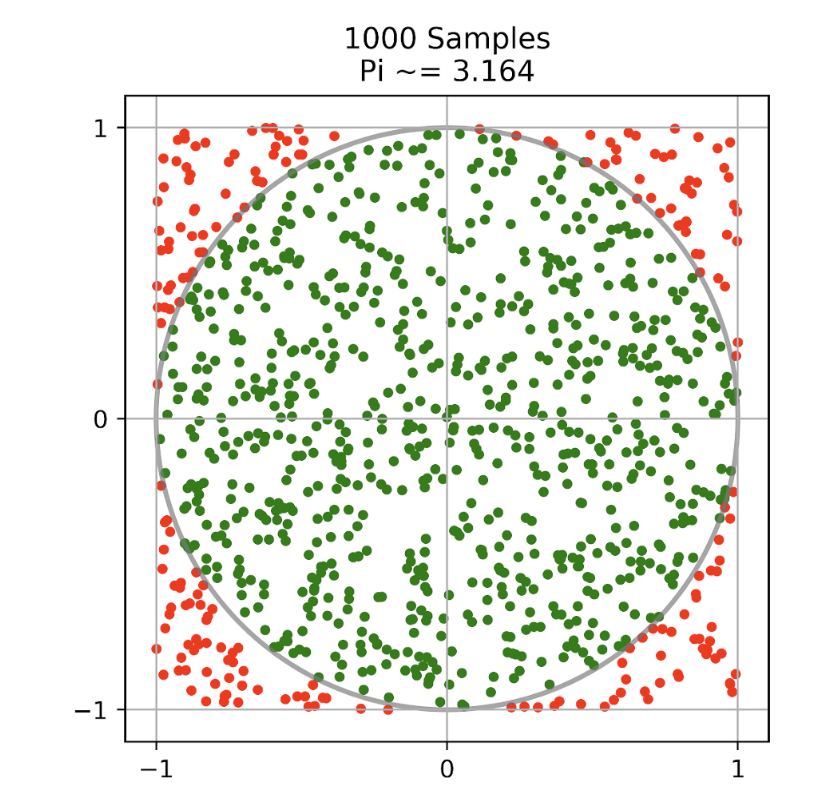
\includegraphics[width=0.4\textwidth]{figuras/monte_carlo_calculo_pi.png}
    \end{center}

    $$
    P(X^2 + Y^2 \le R^2) =
    \frac{\text{Área do círculo}}{\text{Área do quadrado}} =
    \frac{\pi R^2}{(2R)^2} = \frac{\pi}{4}.
    $$

\subsection{Cálculo de Integral}
Seja a integral:
    $$
    \theta = \int_{0}^{1} g(u)\, du.
    $$

Vamos considerar a Distribuição Uniforme em $[a,b]$,
    $$
    f(u) =
    \begin{cases}
    \dfrac{1}{b-a}, & a \le u \le b,\\[6pt]
    0, & \text{caso contrário.}
    \end{cases}
    $$
    
Se $a=0$ e $b=1$, temos a Distribuição Uniforme em $[0,1]$,
    $$
    f(u) =
    \begin{cases}
    1, & 0 \le u \le 1,\\
    0, & \text{caso contrário.}
    \end{cases}
    $$
    
Assim, podemos escrever $\theta$ como:
    $$
    \theta = \int_{0}^{1} 1 \cdot g(u)\, du
    = \int_{0}^{1} f(u)\, g(u)\, du
    = E[g(U)],
    $$
onde $U$ é uma variável aleatória com Distribuição Uniforme em $[0,1]$.

\subsubsection{Integrais Impróprias}
Podemos ainda usar números aleatórios para calcular integrais impróprias, cujos limites de integração são definidos em $[0, \infty)$, isto é,
    $$
    \theta = \int_{0}^{\infty} g(x)\, dx.
    $$

Fazendo uma mudança de variáveis,
    $$
    y = \frac{1}{x+1}
    \implies dy = -\left(\frac{1}{x+1}\right)^{2} dx
    = -y^2 dx
    \implies dx = \frac{dy}{y^2}.
    $$

Note que:
    $$
    \lim_{x \to 0} \frac{1}{x+1} = 1, \quad
    \lim_{x \to \infty} \frac{1}{x+1} = 0.
    $$

Assim,
    $$
    \theta = \int_{0}^{\infty} g(x)\, dx
    = \int_{1}^{0} g\left( \frac{1}{y} - 1 \right) \frac{dy}{y^2}
    = \int_{0}^{1} h(y)\, dy,
    $$
    onde
    $$
    h(y) = \frac{g\left( \frac{1}{y} - 1 \right)}{y^2}.
    $$

\subsubsection{Integrais Múltiplas}
    $$
    \theta = \int_{a}^{b}\!\!\int_{c}^{d} g(x,y)\, dy\, dx,
    $$

Fazemos as transformações:
    $$
    z=\frac{x-a}{\,b-a\,} \;\;\Longrightarrow\;\; x = z(b-a)+a \;\;\Longrightarrow\;\; dx=(b-a)\,dz,
    $$
    $$
    w=\frac{y-c}{\,d-c\,} \;\;\Longrightarrow\;\; y = w(d-c)+c \;\;\Longrightarrow\;\; dy=(d-c)\,dw.
    $$
    
Assim, temos:
    $$
    \theta=\int_{0}^{1}\!\!\int_{0}^{1} h(z,w)\, dz\, dw,
    $$
onde
    $$
    h(z,w)=(b-a)(d-c)\; g\!\big(z(b-a)+a,\; w(d-c)+c\big).
    $$

    Assim:
    $$
    \theta = E\!\left[h(Z,W)\right],
    $$
com $Z,W \sim U(0,1)$ independentes.

\subsection{Simulação de Variáveis Aleatórias}
$X$ é uma variável aleatória com função de distribuição $F_X(x) = P(X \le x)$. Como $F_X$ é estritamente não-decrescente, então:
    $$
    u \le F_X(x) \iff F_X^{-1}(u) \le x,
    $$
onde assumimos que a inversa $F_X^{-1}$ da função $F_X$ existe.

Vamos encontrar a variável aleatória $Y = F_X^{-1}(U)$ que tem a mesma distribuição de $X$,
onde $U$ tem Distribuição Uniforme em $[0,1]$.
Assim, se $F_X(x) = u$, temos:
$$
P(U \le u) = P(U \le F_X(x))
= P(F_X^{-1}(U) \le F_X^{-1}(F_X(x)))
= P(F_X^{-1}(U) \le x) = P(Y \le x) = F_X(x).
$$

Essa igualdade ocorre apenas se $Y = F_X^{-1}(U)$ tem a mesma distribuição de $X$.

Portanto, para simularmos a variável aleatória $X$, geramos $n$ valores $u_1, u_2, \ldots, u_n$, onde $u_i \sim U(0,1)$, $i = 1,2,\ldots,n$, e calculamos $x_i = F_X^{-1}(u_i)$, onde $F_X(x) = P(X \le x)$ é a função de distribuição de $X$. O algoritmo geral é dado por:
\begin{itemize}
    \item Gere um valor $u_i$ a partir da Distribuição Uniforme em $[0,1]$.
    \item Calcule $x_i = F_X^{-1}(u_i)$, onde $F_X(x) = P(X \le x)$ é a distribuição acumulada de $X$.
    \item Repita o processo $n$ vezes para simular $n$ valores de $X$.
\end{itemize}

\section{Análise Exploratória de Dados}
\subsection{Visualização}
\begin{itemize}
    \item Uma das maneiras mais simples de visualizar a distribuição dos dados é através de gráficos de frequência e histogramas;
    \item No caso do histograma, a área sob a curva deve ser igual a 1 e ele é uma aproximação da função densidade de probabilidade;
    \item No caso de variáveis nominais, podemos usar gráficos de barra ou gráficos de setores. Nesse caso, o valor no eixo das abscissas (x) é arbitrário e não deve ser levando em conta;
    \item Outro gráfico importante é o scatterplot, usado quando queremos verificar a relação entre duas variáveis;
    \item Quando temos três variáveis, uma maneira de visualizarmos os dados é considerar um gráfico de calor, sendo que a escala de cores define a terceira variável.
    \item Referência: \url{https://python-graph-gallery.com/}
\end{itemize}

\subsection{Medidas de Posição}
\begin{itemize}
    \item \textbf{Moda}: Uma medida importante de tendência central é a moda, que retorna o elemento mais comum em um conjunto de dados. Geralmente, essa medida é usada para atributos nominais;
    \item \textbf{Média e Mediana}: São medidas de tendência central usadas para dados quantitativos. Assim, a média:
    $$
    \bar{X} = \frac{1}{n} \sum_{i=1}^n x_i
    $$
    A média é altamente sensível a valores extremos, enquanto que a mediana é mais robusta.
    A média é similar à mediana se a distribuição é praticamente simétrica em relação à média. Caso a distribuição não seja simétrica, o mais adequado é usar a mediana como medida central.
    \item \textbf{Percentil}: O percentil é uma medida estatística que indica a posição relativa de um valor dentro de um conjunto de dados, dividindo-o em 100 partes iguais. Ele expressa a porcentagem de valores no conjunto que estão abaixo de um determinado valor.
    \begin{itemize}
        \item Percentil 25 (ou primeiro quartil): 25\% dos valores do conjunto são menores ou iguais a este valor;
        \item Percentil 50 (ou mediana): 50\% dos valores estão abaixo ou no mesmo nível (é o valor central);
        \item Percentil 75 (ou terceiro quartil): 75\% dos valores estão abaixo.
    \end{itemize}
    Para visualizar os quantis, podemos usar o boxplot:
    \begin{figure}[H]
        \centering
        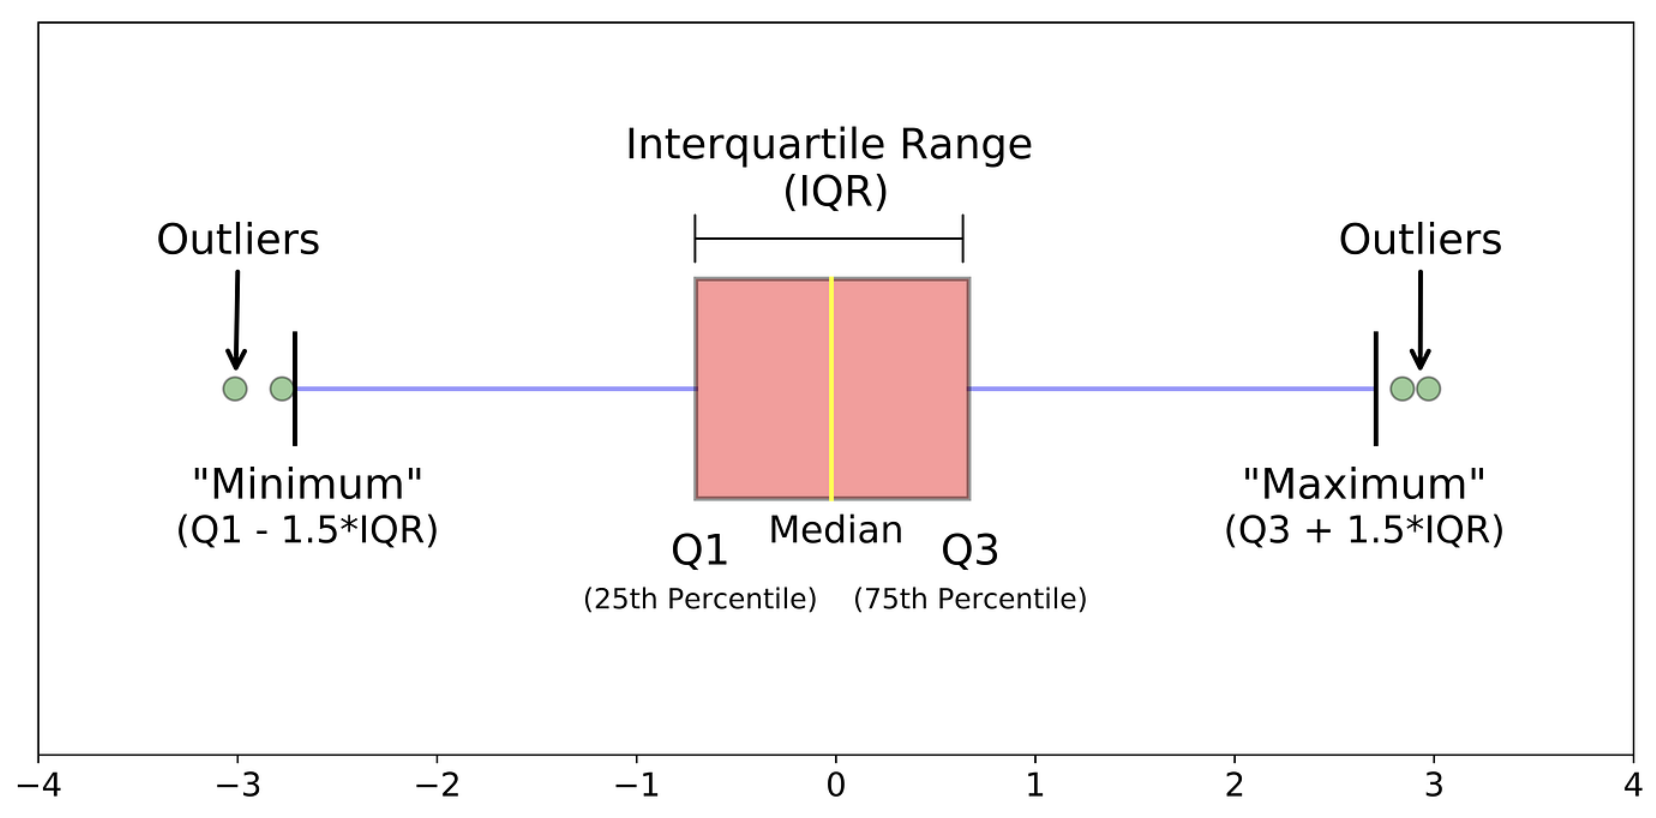
\includegraphics[width=0.8\textwidth]{figuras/boxplot.png}
    \end{figure}
\end{itemize}

\subsection{Medidas de Dispersão}
\begin{itemize}
    \item As medidas de dispersão mais usadas são a variância e o desvio padrão;
    \item A distância interquantil (IQR) também é bastante usada e quantifica a diferença entre o terceiro e primeiro quantil;
    \item Já a amplitude simplesmente mede a diferença entre os valores máximo e mínimo.
\end{itemize}

\subsection{Correlação}
\begin{itemize}
    \item A medida de correlação é importante para analisar a relação entre as variáveis. Se duas variáveis são altamente correlacionadas, é adequado remover uma delas, de modo a reduzir informação redundante nos dados.
    \item \textbf{Correlação de Pearson}: Como apresentado na Seção~\ref{sec:correlacao_pearson};
    \item \textbf{Correlação de Spearman}: A correlação de Spearman mede a associação monotônica entre duas variáveis usando seus ranks em vez dos valores brutos (diferente da de Pearson, que mede relação linear), e sua fórmula é:
    $$
    \rho = 1 - \frac{6 \sum d_i^2}{n(n^2 - 1)}
    $$
    O coeficiente de Spearman nada mais é do que o coeficiente de Pearson aplicado à ordem dos valores.
\end{itemize}

\subsection{Análise dos Componentes Principais}
\begin{itemize}
    \item \textbf{Objetivo}: Reduzir a dimensionalidade dos dados mantendo o máximo possível da variabilidade (informação) original;
    \item \textbf{Centralização dos dados}: Subtrai-se a média de cada variável para que tenham média zero;
    \item \textbf{Cálculo da matriz de covariância (ou de correlação)}: Para entender como as variáveis variam juntas.
    \item \textbf{Autovalores e Autovetores}: Extrai-se os autovetores (direções principais) e autovalores (quantidade de variância explicada) da matriz de covariância;
    \item \textbf{Ordenação}: Classifica-se os autovetores pelo autovalor correspondente, do maior para o menor.
    \item \textbf{Seleção de Componentes}: Escolhe-se os primeiros $k$ autovetores que explicam a maior parte da variância;
    \item \textbf{Projeção dos Dados}: Transforma-se os dados originais para o novo espaço definido pelos $k$ componentes principais.
    \item Para estimarmos o número de componentes para projetarmos os dados, podemos analisar como a variância muda de acordo com o número de componentes.
\end{itemize}

\section{Estimação Pontual}
Definições:
\begin{enumerate}
    \item Um parâmetro é uma medida para descrever uma característica da população;
    \item Uma amostra aleatória é uma coleção de variáveis aleatórias 
    $X_1, X_2, \ldots, X_n$ independentes e identicamente distribuídas;
    \item Seja uma amostra aleatória $X_1, X_2, \ldots, X_n$ de uma população. Uma estatística é uma função de $X_1, X_2, \ldots, X_n$;
    \item Um estimador é uma estatística usada para estimar um parâmetro da população.
\end{enumerate}

\subsection{Função de Verossimilhança}
Seja $X_1, X_2, \ldots, X_n$ uma amostra aleatória obtida de uma distribuição de probabilidade com parâmetros $\theta_1, \ldots, \theta_k$. 
Suponha que observamos $X_1 = x_1, X_2 = x_2, \ldots, X_n = x_n$. 
Então, se as variáveis $X_1, X_2, \ldots, X_n$ são discretas, a função de verossimilhança é definida por:
    $$
    L(\theta; \mathbf{x}) = L(\theta_1, \theta_2, \ldots, \theta_k; x_1, \ldots, x_n) 
    = \prod_{i=1}^n P(X_i = x_i; \theta_1, \theta_2, \ldots, \theta_k).
    $$

Por outro lado, se as variáveis aleatórias são contínuas, então a função de verossimilhança é dada por:
    $$
    L(\theta; \mathbf{x}) = L(\theta_1, \theta_2, \ldots, \theta_k; x_1, \ldots, x_n) 
    = \prod_{i=1}^n f(x_i; \theta_1, \theta_2, \ldots, \theta_k).
    $$

\subsection{Estimador de Máxima Verossimilhança}
Para realizarmos a maximização da função de verossimilhança, precisamos derivar essa função com relação aos parâmetros $\theta$ e igualar o resultado a zero.
    
No entanto, como essa função é definida em termos de um produtório, para facilitar os cálculos, podemos usar a função logaritmo, de forma a transformar os produtos em somas. Assim,   
    $$
    \ell(\theta; \mathbf{x}) = \log \left( L(\theta; \mathbf{x}) \right).
    $$
    
Estamos usando a base $e$ ($\log(x) = \ln(x)$), mas outras bases também podem ser usadas.

O estimador de máxima verossimilhança $\hat{\theta}$ é definido por:
    $$
    \hat{\theta} = \arg\max_{\theta \in \Theta} \, \ell(\theta; \mathbf{x}),
    $$
onde $\Theta$ é o espaço dos parâmetros.

Definições:
\begin{itemize}
    \item Um estimador $\hat{\theta}$ para o parâmetro populacional $\theta$ é não viesado (ou não viciado) se:
        $$
        E[\hat{\theta}] = \theta.
        $$
    \item Um estimador $\hat{\theta}_n = \hat{\theta}_n(X_1, \ldots, X_n)$ é assintoticamente não viesado se
        $$
        \lim_{n \to \infty} E[\hat{\theta}_n] = \theta.
        $$
    \item Uma sequência de estimadores $\hat{\theta}_n = \hat{\theta}_n(X_1, \ldots, X_n)$ é consistente se
        $$
        \lim_{n \to \infty} P\{|\hat{\theta}_n - \theta| > \varepsilon\} = 0,
        \quad \text{para todo } \varepsilon > 0.
        $$
    Em outras palavras, uma sequência de estimadores é consistente se:
        $$
        \begin{cases}
        \lim_{n \to \infty} E[\hat{\theta}_n] = \theta \\
        \lim_{n \to \infty} V[\hat{\theta}_n] = 0
        \end{cases}
        $$
\end{itemize}

Propriedades:
\begin{itemize}
    \item O estimador de máxima verossimilhança é assintoticamente consistente, de modo que ele converge em probabilidade para a quantidade que está sendo estimada, isto é,
        $$
        \lim_{n \to \infty} P\{|\hat{\theta}_n - \theta| > \varepsilon\} = 0,
        $$
    onde $\hat{\theta}_n$ é o estimador obtido para uma amostra de tamanho $n$. Portanto, quando aumentamos o tamanho da amostra, a probabilidade do estimador de estar próximo do parâmetro de população aumenta.
    \item O estimador de máxima verossimilhança é assintoticamente não viesado, isto é,
        $$
        \lim_{n \to \infty} E[\hat{\theta}] = \theta.
        $$
    \item O estimador de máxima verossimilhança é equivarante, ou seja, se $\hat{\theta}$ é o estimador de $\theta$, então $g(\hat{\theta})$ é o estimador de $g(\theta)$
    \item O estimador é assintoticamente normal, isto é,
        $$
        \frac{\hat{\theta} - \theta}{\hat{s}e} \sim \mathcal{N}(0,1),
        $$
    onde
        $$
        \hat{s}e = \sqrt{V(\hat{\theta})},
        $$
    é o erro padrão.
    \item O estimador de máxima verossimilhança é assintoticamente ótimo e eficiente, sendo, para amostras grandes, o estimador que apresenta menor variância dentre todos os estimadores possíveis.
\end{itemize}

\subsubsection{Estimador de Máxima Verossimilhança da Distribuição Normal}
Assim, o Estimador de Máxima Verossimilhança para o modelo normal:
\begin{itemize}
    \item Média $\mu$:
    $$
    \hat{\mu} = \frac{\sum_{i=1}^n X_i}{n} = \bar{X}.
    $$
    \item Variância ($\sigma^2$):
    $$
    \hat{\sigma}^2 = \frac{\sum_{i=1}^n (X_i - \bar{X})^2}{n}.
    $$
\end{itemize}

\subsubsection{Estimador de Máxima Verossimilhança da Distribuição Binomial}
O estimador de verossimilhança do parâmetro $\theta$ para uma Distribuição Binomial com parâmetro $m$ (número de experimentos) e $\theta$ (probabilidade de sucesso) é dado por:
    $$
    \hat{\theta} = \frac{1}{nm} \sum_{i=1}^n X_i.
    $$
    
\subsubsection{Estimador de Máxima Verossimilhança da Distribuição Exponencial}
O estimador de máxima verossimilhança de uma população que segue o modelo exponencial é dado por:
    $$
    \hat{\theta} = \frac{n}{\sum_{i=1}^n x_i}.
    $$

\section{Teorema Central do Limite}
Seja $X$ uma variável aleatória com esperança $E[X] = \mu$ e variância $V(X) = \sigma^2$. Seja $\bar{X}$ a média amostral calculada a partir de $n$ amostras independentes e identicamente distribuídas de $X$, $X_1, X_2, \ldots, X_n$, onde $E[X_i] = \mu$ e $V(X_i) = \sigma^2$, $i = 1, 2, \ldots, n$. 

A distribuição amostral de $\bar{X}$ aproxima-se, para $n$ grande, de uma Distribuição Normal com:
    $$E[\bar{X}] = \mu,$$
    $$V(\bar{X}) = \frac{\sigma^2}{n}.$$


\textbf{Definição equivalente de Lindeberg-Lévy}: Suponha que $\{X_1, X_2, \ldots, X_n\}$ é uma sequência de variáveis aleatórias independentes e identicamente distribuídas com média $E[X_i] = \mu$ e variância $V(X_i) = \sigma^2 < \infty$. Então, quando $n \to \infty$, as variáveis aleatórias $\sqrt{n}(\bar{X}_n - \mu)$ convergem para uma Distribuição Normal $\mathcal{N}(0, \sigma^2)$.  
    $$\sqrt{n}(\bar{X}_n - \mu) \;\;\overset{d}{\longrightarrow}\;\; \mathcal{N}(0, \sigma^2)$$

\textbf{Corolário:} Seja $\{X_1, X_2, \ldots, X_n\}$ uma amostra de uma população $X$ com média $\mu$ e variância $\sigma^2 < \infty$.  Então,
    $$Z = \frac{\bar{X} - \mu}{\sigma / \sqrt{n}} \sim \mathcal{N}(\mu = 0, \sigma^2 = 1)$$

\begin{figure}[H]
    \centering
    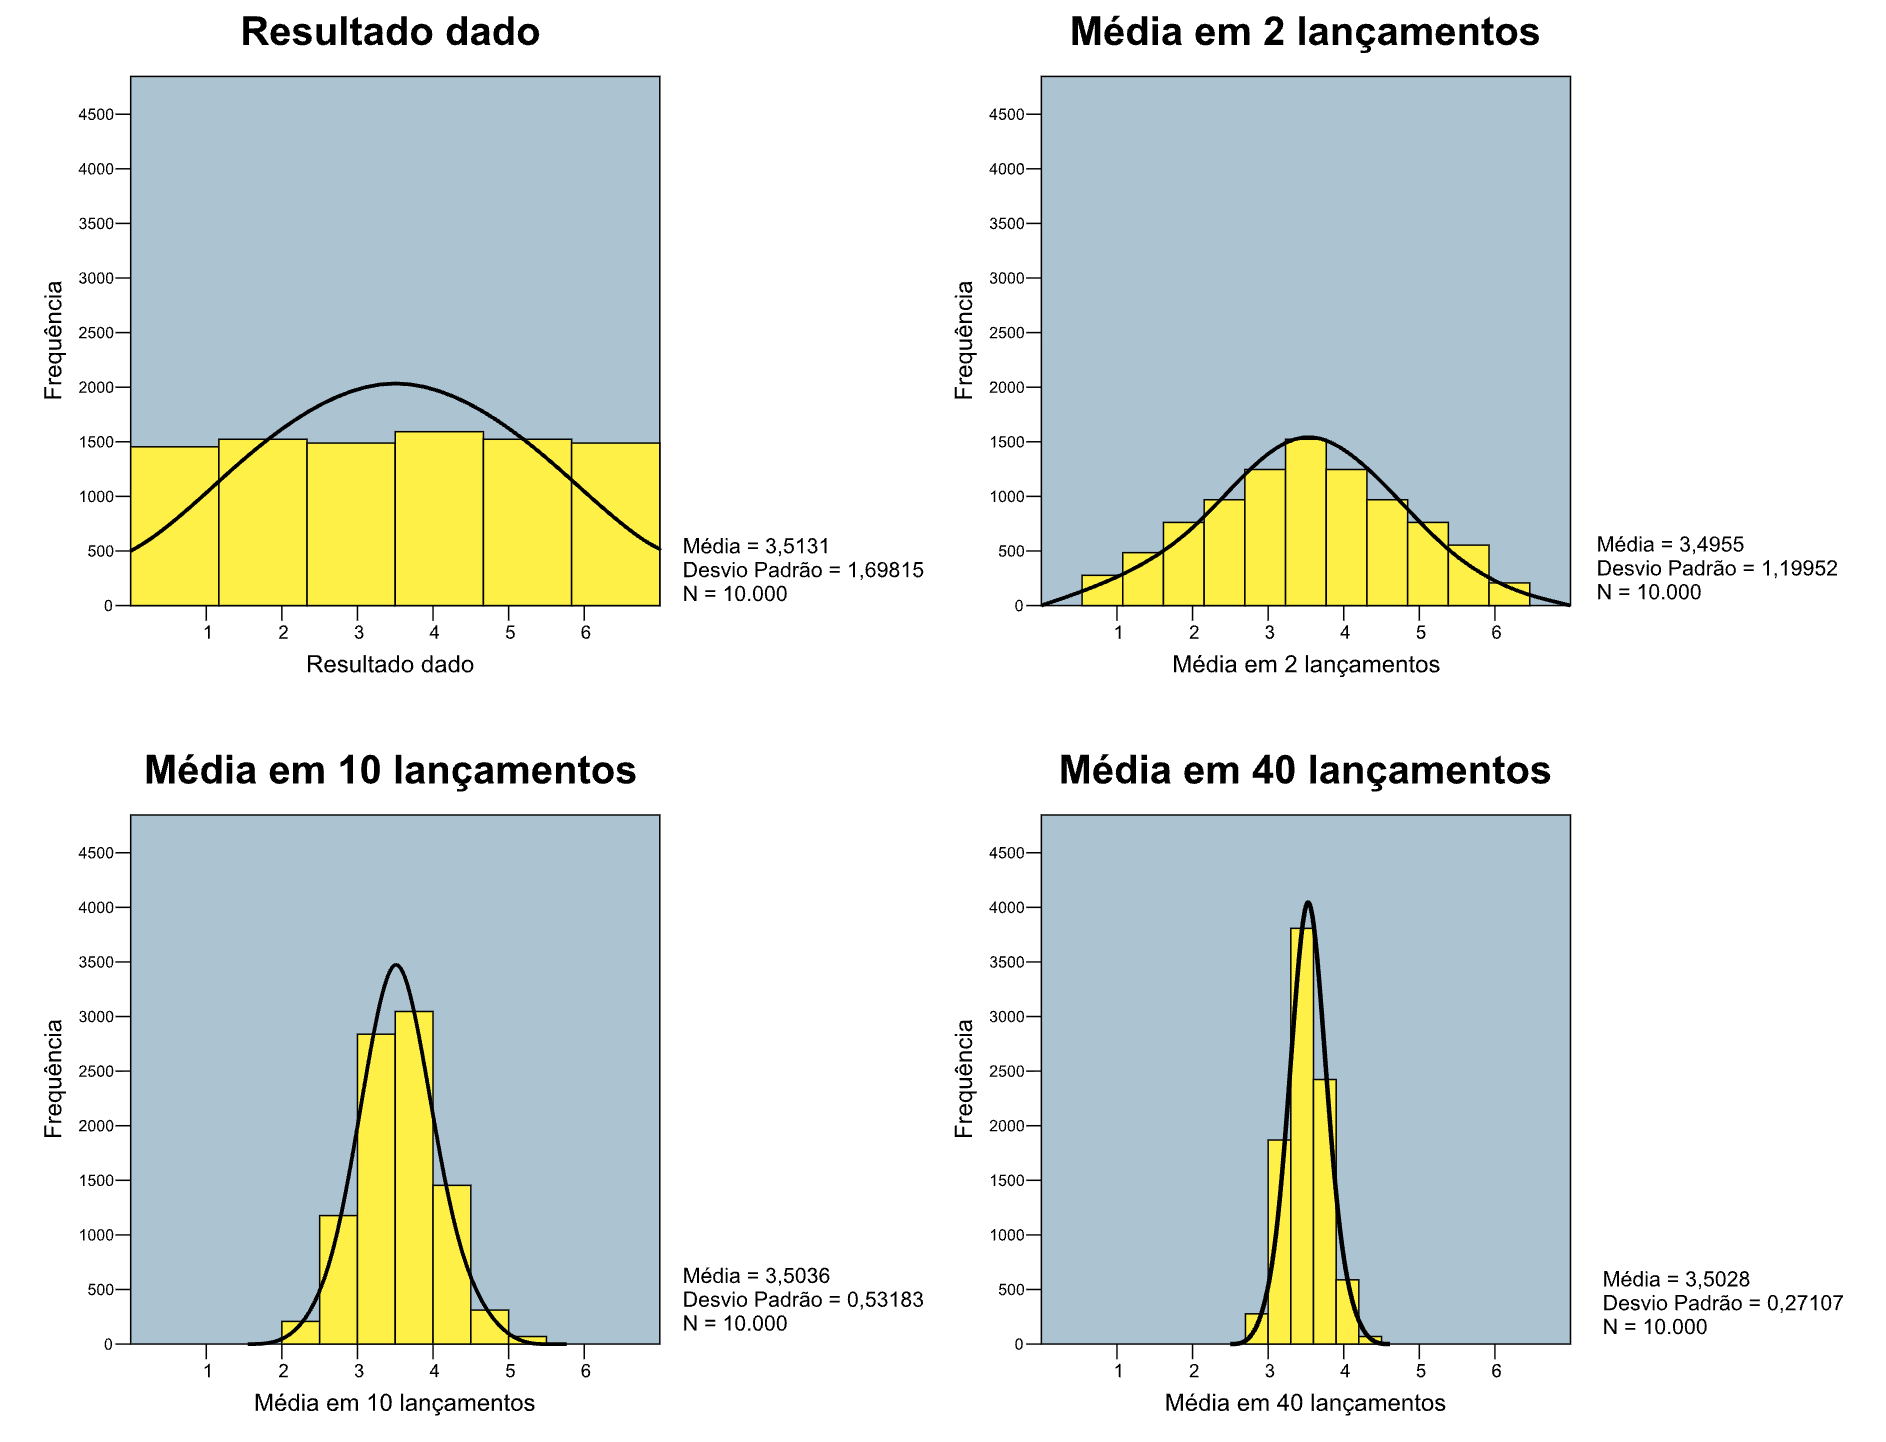
\includegraphics[width=0.85\textwidth]{figuras/teorema_central_limite.png}
    \caption{Teorema Central do Limite.}
    \label{fig:teorema_central_limite}
\end{figure}

No caso em que a variável aleatória é binária, o Teorema Central do Limite pode ser adaptado para o caso de proporções. Seja $\{X_1, X_2, \ldots, X_n\}$ uma amostra aleatória independente e identicamente distribuída onde:
    \[
    \begin{cases}
    P(X_i = 1) = p \\
    P(X_i = 0) = 1 - p.
    \end{cases}
    \]

O número de sucessos é dado pela soma das variáveis aleatórias,
    $$
    S_n = \sum_{i=1}^{n} X_i
    $$

Assim, temos que $\bar{X} = S_n/n$. Com isso, usando os resultados anteriores, obtemos:
    $$
    Z = \frac{\bar{X} - \mu}{\sigma / \sqrt{n}} \sim \mathcal{N}(\mu = 0, \sigma^2 = 1),
    $$
onde $\mu = p$ e $\sigma^2 = p(1 - p)$ são a esperança e variância da Distribuição de Bernoulli, respectivamente. Portanto,
    $$
    Z = \frac{\bar{X} - p}{\sqrt{p(1 - p)/n}} \sim \mathcal{N}(\mu = 0, \sigma^2 = 1)
    $$

\section{Lei dos Grandes Números}
No século XVI, em seu livro sobre jogos de azar, Gerolamo Cardano (1501-1576) afirmou que a acurácia de experimentos estatísticos tende a aumentar com o número de tentativas. Por exemplo, se lançamos uma moeda justa e calculamos a probabilidade de sair cara, essa probabilidade deve ser aproximar cada vez mais do valor 0.5 na medida em que aumentarmos o número de lançamentos.

\textbf{Lei Fraca dos Grandes Números}

Sejam $X_1, X_2, \ldots, X_n$ variáveis aleatórias independentes e identicamente distribuídas com esperança $E[X_i] = \mu < \infty$, $i = 1, 2, \ldots, n$. Seja $\epsilon > 0$. Então,

$$\lim_{n \to \infty} P(|\bar{X} - \mu| \geq \epsilon) = 0,$$
    onde $\bar{X} = \sum_{i=1}^n X_i / n$ é a média amostral.

Ou seja:
    $$\lim_{n \to \infty} \sum_{i=1}^n \frac{X_i}{n} = \mu = E[X].$$

\textbf{Lei Forte dos Grandes Números}

Seja $S_n = \sum_{i=1}^n X_i$ a soma de $n$ variáveis aleatórias independentes e identicamente distribuídas, cada uma com média $E[X_i] = \mu$, $i = 1, 2, \ldots, n$. Seja ainda $\bar{X} = S_n/n$. Então,
    $$P\left(\lim_{n \to \infty} \bar{X} = \mu\right) = 1.$$

Em resumo, podemos dizer que na Lei Fraca dos Grandes Números, há uma alta probabilidade de que $\bar{X}_n$ se aproxime de $E[X] = \mu$ quando $n$ cresce. Essa propriedade é chamada de convergência fraca. Já no caso da Lei Forte dos Grandes Números, pode-se afirmar, com certeza, que a média amostral convergirá para a média $\mu$ quando $n \to \infty$. Esse tipo de convergência é chamada de “convergência quase certa”.

\section{Desigualdade de Markov}
Seja $X$ uma variável aleatória com valores não-negativos. Então, para $\delta > 0$, temos:
    $$
    P(X \geq \delta) \leq \frac{E[X]}{\delta}, \quad E[X] < \infty.
    $$

\section{Desigualdade de Chebyshev}
Seja X uma variável aleatória com esperança $E[X] = \mu$ variância $V(X) = \sigma^2$.
Então, para todo $\delta > 0$,
    $$
    P(|X - \mu| \geq \delta) \leq \frac{\sigma^2}{\delta^2}
    $$

\section{Desigualdade de Jensen}
Seja $g(X)$ uma função convexa de uma variável aleatória $X$. Então,
    $$
    E[g(X)] \geq g(E[X])
    $$

\section{Função Geratriz de Momentos}
Seja $X$ uma variável aleatória discreta ou contínua. A função geratriz de momentos de $X$ é definida por:
    $$
    M_X(t) = E[e^{tX}].
    $$

Seja $M_X(t)$ a função geratriz de momentos da variável aleatória $X$. Então:
    $$
    \frac{d^n}{dt^n} M_X(t) \bigg|_{t=0} = E[X^n].
    $$

Sejam $X$ e $Y$ variáveis aleatórias independentes. Então:
    $$
    M_{X+Y}(t) = M_X(t) M_Y(t)
    $$

Sejam $X_1, X_2, \ldots, X_n$ variáveis aleatórias independentes. Então:
    $$
    M_{X_1+X_2+\ldots+X_n}(t) = M_{X_1}(t) M_{X_2}(t) \ldots M_{X_n}(t)
    $$

\section{Intervalos de Confiança}
\begin{itemize}
    \item Como ocorre flutuação estatística de uma amostra para outra, para caracterizarmos um estimador, é mais adequado definirmos um intervalo de confiança do que usar um único valor estimado.
    \item O intervalo de confiança é construído levando-se em consideração a variabilidade dos dados amostrais e o tamanho da amostra. Ele fornece uma faixa de valores plausíveis para o parâmetro populacional com base na amostra coletada.
\end{itemize}

O intervalo de confiança de $\gamma = (1 - \alpha)100\%$ para a média populacional $\mu$ de uma população com variância conhecida $\sigma^2$ é dado por:
    $$
    IC(\mu; 1 - \alpha) =
    \left[
    \bar{X}_n - z_{\alpha/2}\frac{\sigma}{\sqrt{n}};\ 
    \bar{X}_n + z_{\alpha/2}\frac{\sigma}{\sqrt{n}}
    \right].
    $$

\begin{figure}[H]
    \centering
    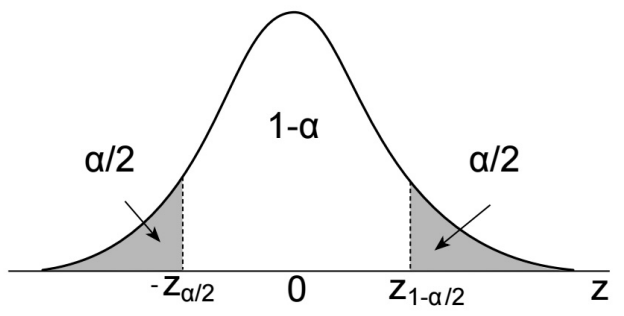
\includegraphics[width=0.6\textwidth]{figuras/intervalo_confianca.png}
    \caption{Intervalo de Confiança.}
    \label{fig:intervalo_confianca}
\end{figure}

Notem que o nível de confiança, o tamanho da amostra e a variância da população influenciam no comprimento do intervalo.
Para um nível de confiança fixo, o comprimento do intervalo diminui de acordo com o tamanho da amostra $n$.
Em outras palavras, quanto maior a amostra, menor o comprimento do intervalo, o que reduz a incerteza nos resultados.

Observem que para calcular o intervalo de confiança, precisamos conhecer o desvio padrão da população. No entanto, na maioria dos problemas de inferência estatística, não temos acesso ao valor desse parâmetro, o que é esperado, já que também não conhecemos a média. Nessas situações, devemos considerar o desvio padrão amostral, que é um estimador não viesado e consistente para o desvio padrão da população. 
O desvio padrão amostral é definido por:
    $$
    S_n = \sqrt{\frac{1}{n-1} \sum_{i=1}^n (X_i - \bar{X}_n)^2}
    $$
Para calcularmos o intervalo de confiança, substituímos o desvio padrão populacional pelo amostral e usamos o teorema a seguir.

A estatística
    $$
    T = \frac{\bar{X}_n - \mu}{S_n / \sqrt{n}}
    $$
possui Distribuição t de Student com $n - 1$ graus de liberdade. Similar ao $Z$, mas usado quando $n\leq50$.

\begin{figure}[H]
    \centering
    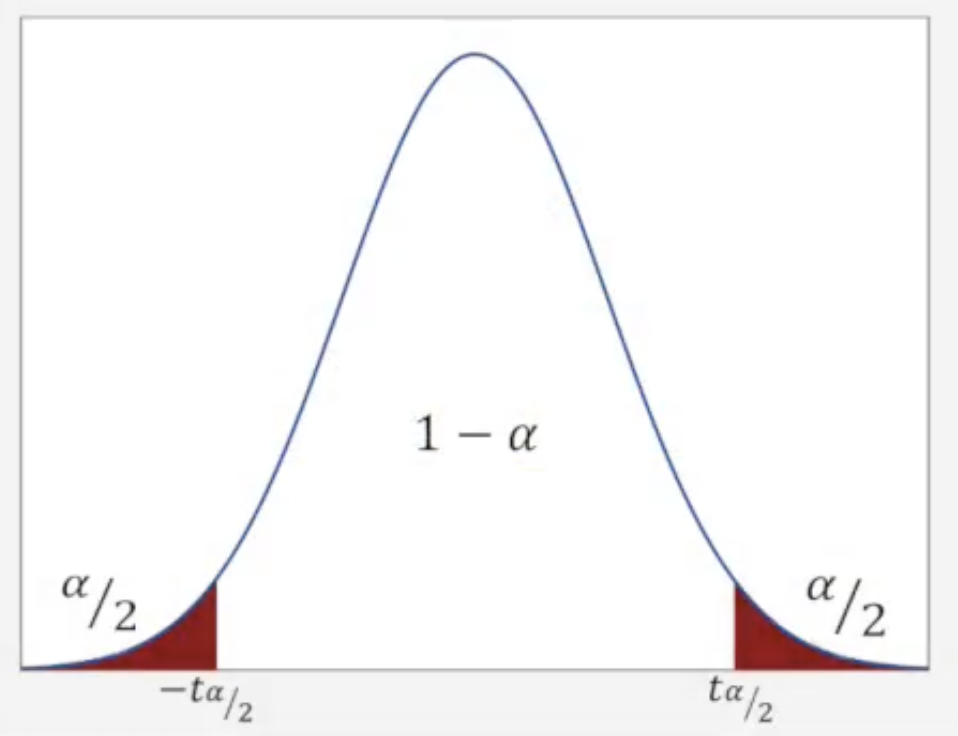
\includegraphics[width=0.6\textwidth]{figuras/intervalo_confianca_t_student.png}
    \caption{Intervalo de Confiança com t de Student.}
    \label{fig:intervalo_confianca_t_student}
\end{figure}

O intervalo de confiança de $\gamma = (1 - \alpha)100\%$ para a média populacional $\mu$, de uma população com variância desconhecida, é dado por:
    $$
    IC(\mu; 1 - \alpha) = 
    \left[
    \bar{X}_n - t_{\alpha/2, n-1}\frac{S_n}{\sqrt{n}}; 
    \bar{X}_n + t_{\alpha/2, n-1}\frac{S_n}{\sqrt{n}}
    \right]
    $$

Se o tamanho da população $n$ for grande (usualmente maior do que 50), devemos usar a Distribuição Normal padronizada e, nesse caso,
    $$
    IC(\mu; 1 - \alpha) = 
    \left[
    \bar{X}_n - z_{\alpha/2}\frac{S_n}{\sqrt{n}}; 
    \bar{X}_n + z_{\alpha/2}\frac{S_n}{\sqrt{n}}
    \right]
    $$

A tabela Normal pode ser acessada através do link \url{https://en.wikipedia.org/wiki/Student%27s_t-distribution#Table_of_selected_values}.

\begin{figure}[H]
    \centering
    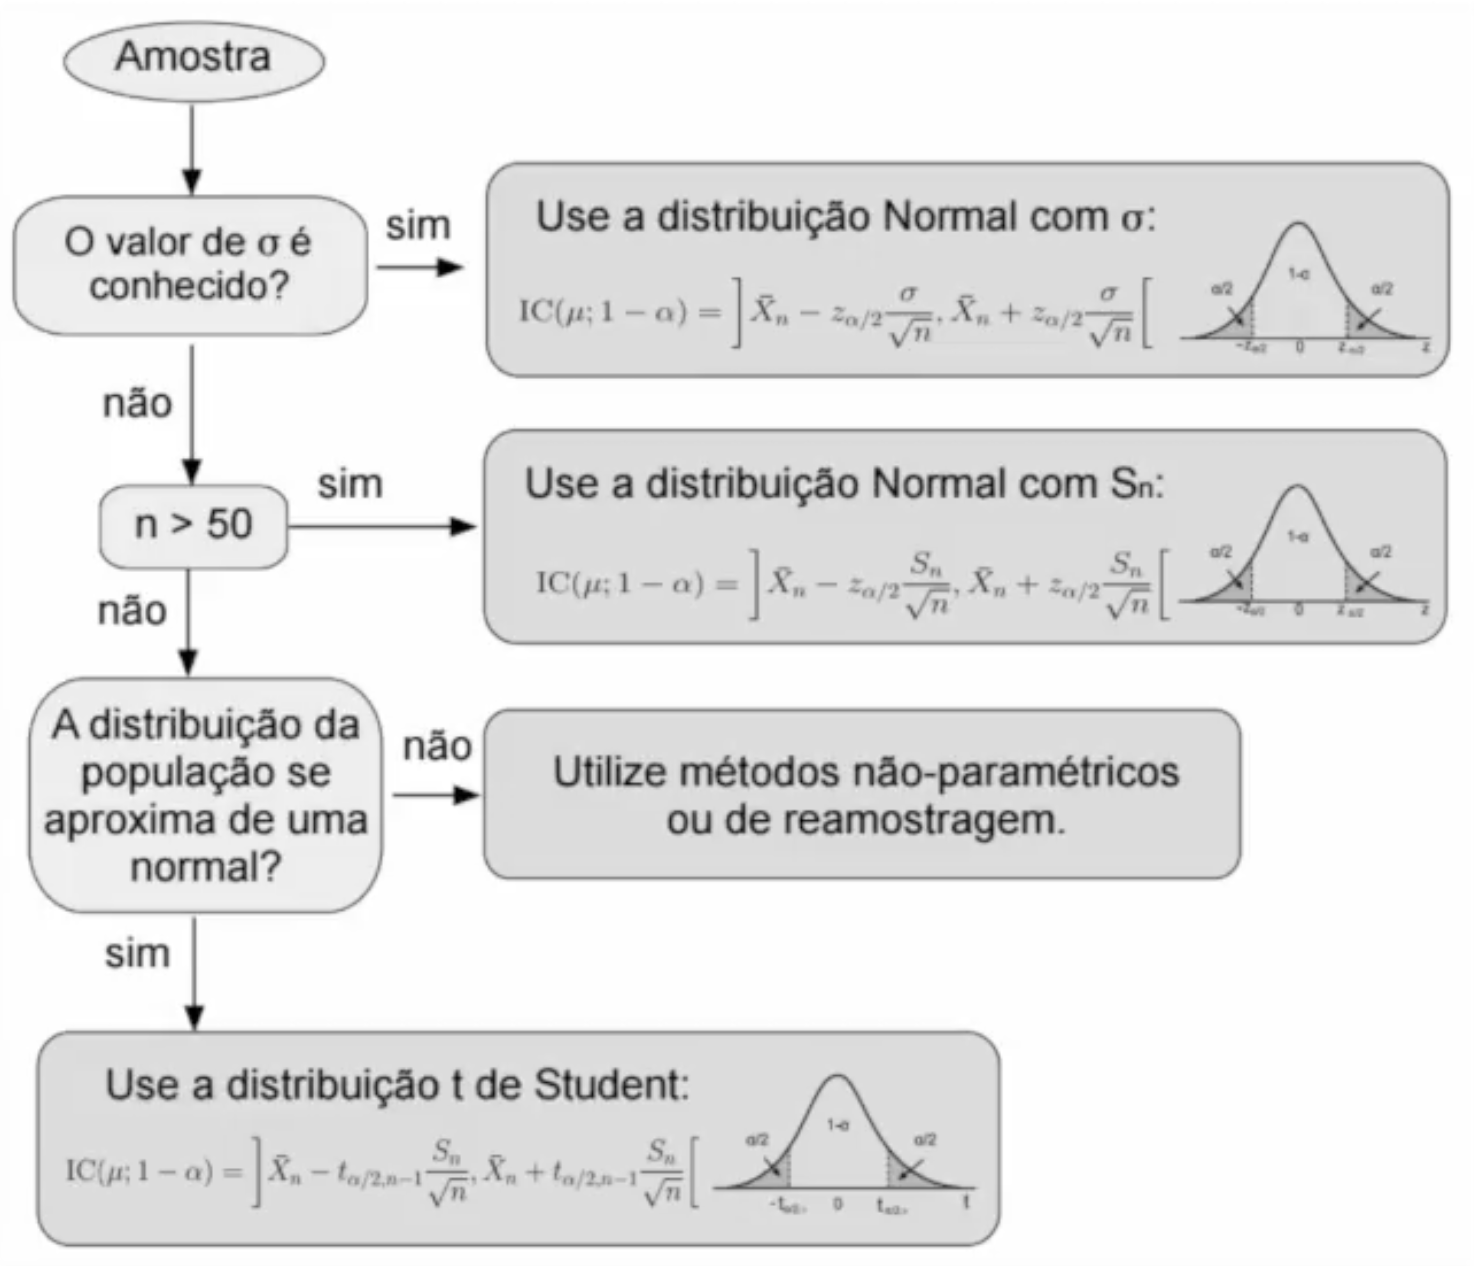
\includegraphics[width=0.6\textwidth]{figuras/intervalo_confianca_fluxograma.png}
    \caption{Fluxograma para cálculo do Intervalo de Confiança.}
    \label{fig:intervalo_confianca_fluxograma}
\end{figure}

Além da média populacional, podemos calcular o intervalo de confiança para uma proporção. Nesse caso, vimos que pelo Teorema Central do Limite, que a variável aleatória $Z$ é definida por:
    $$
    Z = \frac{\hat{p} - p}{\sqrt{p(1-p)/n}} \sim \mathcal{N}(0,1),
    $$
onde $p$ é a proporção de elementos da população que possuem uma certa característica. Seja a variável aleatória $X_i = 1$ se a observação $i$, extraída dessa população, possui uma certa característica, ou $X_i = 0$, caso contrário. Assim, temos que a proporção amostral, para uma amostra de tamanho $n$, é dada por:
    $$
    \hat{p} = \frac{Y_n}{n},
    $$
onde $Y_n = X_1 + X_2 + \dots + X_n$ é o número de observações que possuem a característica na amostra. Notem que $Y_n$ tem Distribuição Binomial.

O intervalo de confiança de $\gamma = (1 - \alpha)100\%$ para a proporção populacional $p$ é dado por:
    $$
    IC(p; 1-\alpha) = 
    \left[
    \hat{p} - z_{\alpha/2}\frac{\sqrt{\hat{p}(1-\hat{p})}}{\sqrt{n}} \;;\;
    \hat{p} + z_{\alpha/2}\frac{\sqrt{\hat{p}(1-\hat{p})}}{\sqrt{n}}
    \right].
    $$

Uma outra opção para calcularmos o intervalo de confiança para a proporção populacional, é usar o fato de que $p(1-p) \leq 1/4$. Ou seja,
    $$
    \frac{p(1-p)}{n} \leq \frac{1}{4n}.
    $$
    $$
    \frac{\sqrt{p(1-p)}}{\sqrt{n}} \leq \frac{\sqrt{1}}{\sqrt{4n}} = \frac{1}{\sqrt{4n}}.
    $$

Substituindo esse resultado na definição anterior, podemos calcular o intervalo, chamado conservador, conforme definido a seguir.

\textbf{Definição: (IC conservador)} O intervalo de confiança de 
    $\gamma = (1-\alpha)100\%$ para a proporção populacional $p$ é dado por:
    $$
    IC(p; 1-\alpha) = 
    \left[
    \hat{p} - \frac{z_{\alpha/2}}{\sqrt{4n}} \, ; \,
    \hat{p} + \frac{z_{\alpha/2}}{\sqrt{4n}}
    \right].
    $$

\subsection{\textit{Bootstraping}}
\begin{itemize}
    \item No caso em que a população não se aproxima de uma Distribuição Normal, precisamos usar métodos de reamostragem ou não paramétricos.
    \item Um método de reamostragem importante é chamado \textit{bootstrapping}, que foi proposto por Bradley Efron em 1979, usa reamostragem dos dados.
    \item A partir dessas amostras, calculamos o intervalo de confiança, que pode ser obtido de diversas maneiras. Se temos $n$ observações coletadas, amostramos $n$ elementos desses dados com reposição.
    \item Para cada amostra obtida, calculamos um estimador $\hat{\theta}$, como a média ou desvio padrão amostral. Considerando várias amostras, podemos construir a distribuição de probabilidade do estimador e, assim, estimar o intervalo de confiança para o parâmetro de interesse.
\end{itemize}

Assim, de maneira geral, para calculamos o intervalo de confiança com o método \textit{bootstrapping} usamos os seguintes passos:
\begin{itemize}
    \item Temos uma amostra aleatória $X$ de tamanho $n$ e objetivamos criar um intervalo de confiança para o estimador $\hat{\theta}$.
    \item Repetimos para $10^4$ ou mais vezes:
    \begin{itemize}
        \item Selecione $n$ elementos de $X$ com reposição.
        \item Calcule e armazene o valor de $\hat{\theta}$.
    \end{itemize}
    \item A partir dos dados armazenados, construa um histograma para $\hat{\theta}$.
    \item Se a distribuição obtida é aproximadamente simétrica, construa o intervalo de confiança de $(1-\alpha)100\%$ encontrando os percentis, de modo que a proporção de observações entre os percentis seja $1-\alpha$.
\end{itemize}

% \section{Testes de Hipótese}

\end{document}
